\documentclass[aspectratio=169,11pt]{beamer}

% Shared style (ib-tutorials.sty at the repo root).
\makeatletter\def\input@path{{./}{../}}\makeatother
\usepackage{ib-tutorials}

\usepackage[utf8]{inputenc}
\usepackage{amsmath,amssymb}
\usepackage{booktabs}
\usepackage{array}
\newcolumntype{L}[1]{>{\raggedright\arraybackslash}p{#1}}
\usepackage{graphicx}
\graphicspath{{../pictures/2-ib2d/}{pictures/2-ib2d/}}
\usepackage{xcolor}
\usepackage{listings}
\usepackage{tikz}
\usetikzlibrary{arrows.meta,positioning,shapes.geometric,fit,calc}
\usepackage{hyperref}

\newcommand{\sourcecredit}[1]{\vfill\hfill{\tiny\textcolor{DarkGray}{#1}}}
\newcommand{\gui}[1]{\textsf{\textbf{#1}}}

\lstset{
  basicstyle=\ttfamily\scriptsize\color{BlackGray},
  keywordstyle=\color{NavyBlue}\bfseries,
  commentstyle=\color{DarkGray}\itshape,
  stringstyle=\color{OliveGreen},
  showstringspaces=false,
  columns=fullflexible,
  keepspaces=true,
  breaklines=true,
  frame=single,
  framerule=0.4pt,
  rulecolor=\color{LightGray},
  backgroundcolor=\color{LightGray!30},
  xleftmargin=0.25em,
  xrightmargin=0.25em
}
\lstdefinestyle{shell}{morecomment=[l]{\#}}
\lstdefinestyle{input}{morecomment=[l]{\%}}
\lstdefinestyle{plain}{}
\lstdefinestyle{py}{language=Python}
\lstdefinestyle{tiny}{basicstyle=\ttfamily\tiny\color{BlackGray}}

\title[The IB2d practical; VisIt for IB2d]{The IB2d practical, and VisIt for IB2d}
\subtitle{Run the rubber band in MATLAB or Python and watch it; open the \code{.vtk} output in VisIt step by step (points, velocity vectors, vorticity, the time slider, a movie); the forces on the structure; four more examples to run, and two to read}
\author[Miller]{Laura A. Miller}
\institute[UArizona]{Department of Mathematics, University of Arizona}
\date{Using IB Software \textbullet\ Part II \textbullet\ Chapter 4b}

\begin{document}

% ---------------------------------------------------------------- title
\begin{frame}[plain]
\maketutorialtitlepanel{%
\begin{tikzpicture}[scale=0.95]
  \draw[DarkGray,thick] (0,0) rectangle (4,4);
  \fill[NavyBlue!25] (0.5,1.2) rectangle (1.6,2.8); \fill[RubineRed!25] (2.4,1.2) rectangle (3.5,2.8);
  \draw[BlackGray,very thick] (2,2) ellipse (0.9 and 1.5);
  \foreach \a in {0,20,...,340} {\fill[BlackGray] ({2+0.9*cos(\a)},{2+1.5*sin(\a)}) circle (1.5pt);}
  \node[font=\tiny,DarkGray,anchor=south] at (2,0.15) {Omega.*.vtk + lagsPts.*.vtk};
\end{tikzpicture}}
\end{frame}

% ---------------------------------------------------------------- goals, sources
\begin{frame}{What you will be able to do after this chapter}
\label{fr:goals}
\footnotesize
\begin{itemize}\setlength{\itemsep}{0pt}
  \item Run the rubber-band example in MATLAB (and watch its figure) or in Python, and know what each run leaves behind.
  \item Open IB2d's output in VisIt from scratch: the points, the velocity vectors, the vorticity, all three together, advancing in time; make them look right (point size, limits, nodal, opacity); zoom; save a picture and a movie.
  \item Know the two ways IB2d's files differ from IBAMR's in VisIt (one file per dump and per variable, grouped as a ``database''; MATLAB's files carry a time stamp, Python's do not), and what VisIt asks because of it (the ``Index'' correlation).
  \item Read the forces on the structure (\code{hier\_IB2d\_data}) and plot one number against time.
  \item Run four more Python examples (porous band, heart tube with muscles, the impedance pump with tracers, a beam with target points) and read two MATLAB ones (the swimmer, the leaf) that use the update functions of chapter 4c.
\end{itemize}
\begin{punchbox}
\footnotesize Every VisIt step was repeated headlessly in VisIt 3.5.0 on the Python run's output (\code{wsl/final/visit\_ch4b.sh}); most windows shown are the 2024 practical's (VisIt 3.4.1 on Windows), which look the same in 3.5; four are older VisIt 2.5.2 windows on a Mac that the practical reused (the first File open window, the zoom and the Save-movie screens). The extra examples were run in October 2026 (Python 3.12, numba 0.68); the MATLAB-only ones are described from their files and the 2024 pictures.
\end{punchbox}
\end{frame}

\begin{frame}{Where this chapter comes from}
\label{fr:sources}
\footnotesize
\begin{itemize}
  \item \al{``IB2d Practical'' (2024, 38 slides, 25 screenshots):} the run in MATLAB, the files, then VisIt 3.4.1 step by step on the rubber band (preferences, open the points, mesh, point size, open \code{u}, vectors, the correlation prompt, advance, vorticity, limits, play, zoom, movie), two exercises, and two bigger MATLAB examples (the swimmer, the leaf). The only VisIt-3 walk-through for IB2d; this chapter follows its order.
  \item \al{``ib2d part 2'' (Lecture 10, 2021, edited 2023, 32 slides):} MATLAB vs Python, the ``suggestions to improve'' slides (limits at 25\,\%, nodal, 8000 vectors, constant colour, annotations off, legends, sessions, movies as PNG frames joined in VirtualDub or QuickTime), and the sawtooth that chapter 4c takes up.
  \item \al{``A quick intro to ib2d'' (Lecture 9), slides 31--51:} the VisIt 2.5.2 walk-through written for IBAMR's files (\code{lag\_data.visit}, \code{dumps.visit}) and reused for IB2d; chapter 26 is its home.
  \item Nick Battista's video tutorial 4 (VisIt for IB2d; \url{https://youtu.be/4D4ruXbeCiQ}).
  \item The runs of October 2026 (\code{wsl/final/ib2d\_pyrun*.sh}, \code{ib2d\_pump2.sh}) and the headless VisIt script \code{visit\_ch4b.sh}.
\end{itemize}
What is new here: the headless check of every step in 3.5, the time-stamp difference between the MATLAB and Python writers, the forces plot, the four Python runs with their timings, the tracer-example fix, and the pointers to chapters 26, 30, 32 and 33 for everything VisIt does beyond this walk-through.
\end{frame}

% ---------------------------------------------------------------- part A: the run
\begin{frame}[fragile]{The run, in MATLAB}
\label{fr:runmat}
\begin{columns}[T]
\column{0.5\textwidth}
\footnotesize
Open MATLAB, go to the folder and type the name of the main file:
\begin{lstlisting}[style=plain]
>> cd matIB2d/Examples/Example_Standard_Rubberband/Rubberband_with_Springs
>> main2d
\end{lstlisting}
\begin{itemize}
  \item A figure window opens with three panels (\code{plot\_Matlab = 1}): the Lagrangian points, the vorticity (filled contours) and the velocity (arrows), redrawn at every dump. The picture is the 2024 practical's: ``a rubber band oscillating in a fluid''.
  \item The console prints the banner, ``FIBER MODEL INCLUDES'', then \code{Current Time(s)} at every dump (chapter 4a).
  \item 1500 steps at $32 \times 32$: well under a minute, most of it the figure. Set \code{plot\_Matlab = 0} for a batch run and look at the output in VisIt instead.
\end{itemize}
\column{0.48\textwidth}
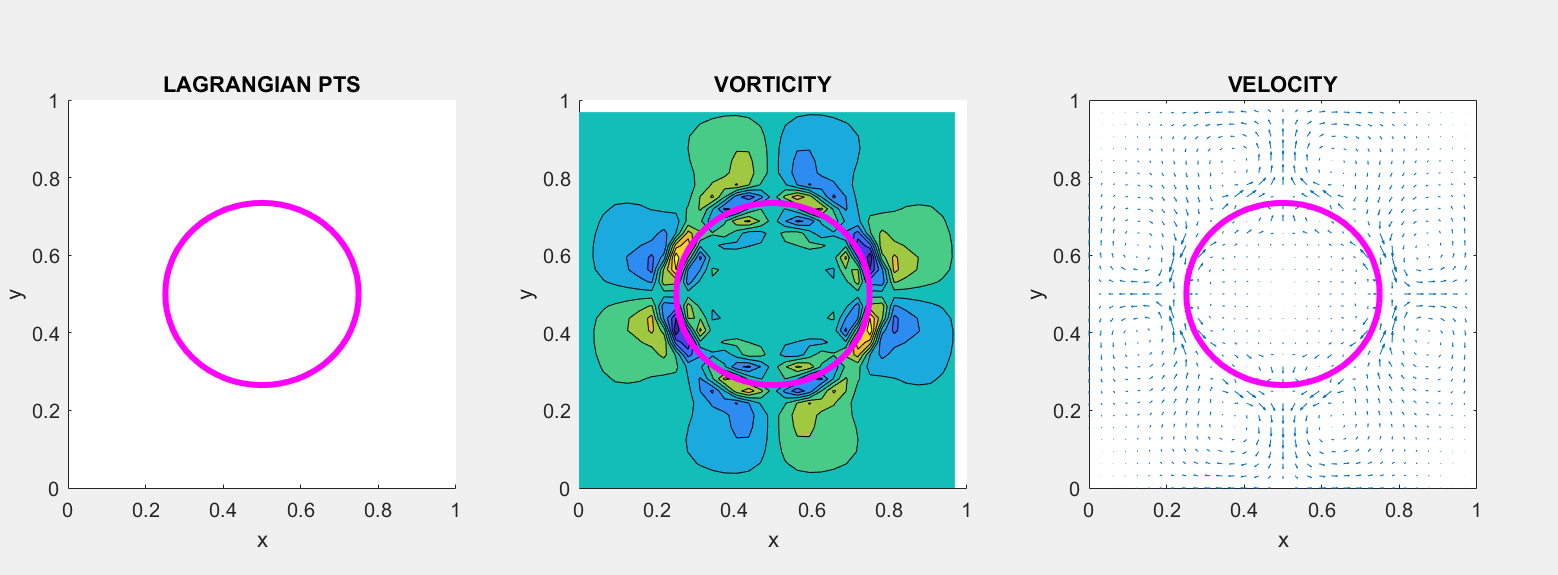
\includegraphics[width=0.95\textwidth]{ch4b-ibp-s03-matlab-run.png}
\scriptsize The MATLAB figure during the run (2024 practical): points, vorticity, velocity. MATLAB R2020a and R2020b cannot draw it (the README names only those two).
\end{columns}
\end{frame}

\begin{frame}[fragile]{The run, in Python; what is left behind}
\label{fr:runpy}
\begin{columns}[T]
\column{0.5\textwidth}
\begin{lstlisting}[style=shell]
cd pyIB2d/Examples/Rubberband_with_Springs
python3 main2d.py          # 3.9 s on a desktop PC, plotting off
ls viz_IB2d | head -3      # Omega.0000.vtk ... (uppercase names sort first)
ls viz_IB2d | wc -l        # 456 files: 76 dumps x 6
ls hier_IB2d_data | wc -l  # 228: fX_Lag, fY_Lag, fMag per dump
\end{lstlisting}
\footnotesize
\begin{itemize}
  \item With \code{plot\_Matlab = 1} the Python version opens a matplotlib window with five panels (its \code{input2d} has every \code{plot\_*} flag on); on a machine without a display set it to 0 (or \code{MPLBACKEND=Agg}).
  \item The same files appear in both versions, with one difference that matters in VisIt: \al{the MATLAB writer stamps each file with its time} (VisIt shows \code{Time: 0.02} for dump 1), \al{the Python writer does not} (VisIt shows the state index: 0, 1, 2, \ldots). Chapter 4a, slide on the output, has the file layout.
\end{itemize}
\column{0.48\textwidth}
\footnotesize
\begin{itemize}
  \item \code{viz\_IB2d/}: \code{lagsPts} (the points), \code{lagPtsConnect} (the points joined along the springs), \code{Omega}, \code{P}, \code{uMag}, \code{u} (vectors), and \code{uX}, \code{uY}, \code{fX}, \code{fY}, \code{fMag}, \code{tracer}, \code{concentration} when their flags or models are on.
  \item \code{hier\_IB2d\_data/}: the force on every point, as \code{fX\_Lag}, \code{fY\_Lag}, \code{fMag} (and \code{fNorm}, \code{fTan} from the MATLAB writer for structures of more than five points; the Python writer has the same branch but tests the wrong array dimension and never writes them, a third item for the note to the repository).
  \item Every file is a dump number: \code{.0000} is $t = 0$, and dump $k$ is $t = k \times$ \code{print\_dump} $\times \Delta t$ ($0.02$ s apart here).
  \item A second run in the same folder overwrites these files one by one; copy the folder, or delete the two output folders, before a new run.
\end{itemize}
\end{columns}
\end{frame}

% ---------------------------------------------------------------- part B: VisIt
\begin{frame}{VisIt for IB2d: what is different from the IBAMR walk-through}
\label{fr:diff}
\small
Chapter 26 opens an IBAMR run (\code{lag\_data.visit}, \code{dumps.visit}: one list file each). IB2d writes \al{one file per dump and per variable}, so:
\begin{itemize}
  \item VisIt's file panel groups the numbered files itself: \gui{File grouping: Smart} shows \code{lagsPts.*.vtk database (76 total files)}, and that ``database'' is what you open. One database per variable: \code{Omega.*.vtk database}, \code{u.*.vtk database}, \ldots
  \item Each database has its own time slider. When a second one is added to the plots, VisIt asks \gui{Would you like to create a ``Index'' database correlation for the following databases?}: say \gui{Yes}, and the sliders move together, state by state (slide \ref{fr:correlate}).
  \item The meshes are all called \code{mesh}; the scalar in the \code{Omega} files is \code{Omega}, the vector in the \code{u} files is \code{u}, the forces in \code{hier\_IB2d\_data} are \code{fMag}, \code{fX\_Lag}, \code{fY\_Lag} on the points.
  \item There are no AMR patches to hide, no \code{U\_x}/\code{U\_y} components to choose, no levels: a $32 \times 32$ uniform grid with the periodic edges.
  \item Everything else (plot attributes, annotations, sessions, saving windows, movies, the CLI) is the same program: chapters 26, 30 and 32 apply unchanged.
\end{itemize}
The steps below are the 2024 practical's, checked in VisIt 3.5.0.
\end{frame}

\begin{frame}{Step 0: install VisIt, set one preference}
\label{fr:install}
\begin{columns}[T]
\column{0.56\textwidth}
\small
\begin{itemize}\setlength{\itemsep}{0pt}
  \item VisIt is free (Lawrence Livermore): \url{https://visit-dav.github.io/visit-website/}; installers for Windows, macOS and Linux. Part V uses 3.5.0; the 2024 practical used 3.4.1 and the windows are the same.
  \item On a Mac with a recent macOS, VisIt may refuse to list files (``The MetaData server running on localhost could not get the file list for the current directory''): start it from the terminal, from the folder you want to open, with \code{/Applications/VisIt.app/Contents/}\allowbreak\code{Resources/bin/visit -gui} (the IB2d README's workaround).
  \item \gui{Options $\to$ Preferences}: untick \gui{Enable warning message popups}. The practical's reason: ``when we start saving movies, a pop-up will spring up every time-step''.
\end{itemize}
\column{0.42\textwidth}
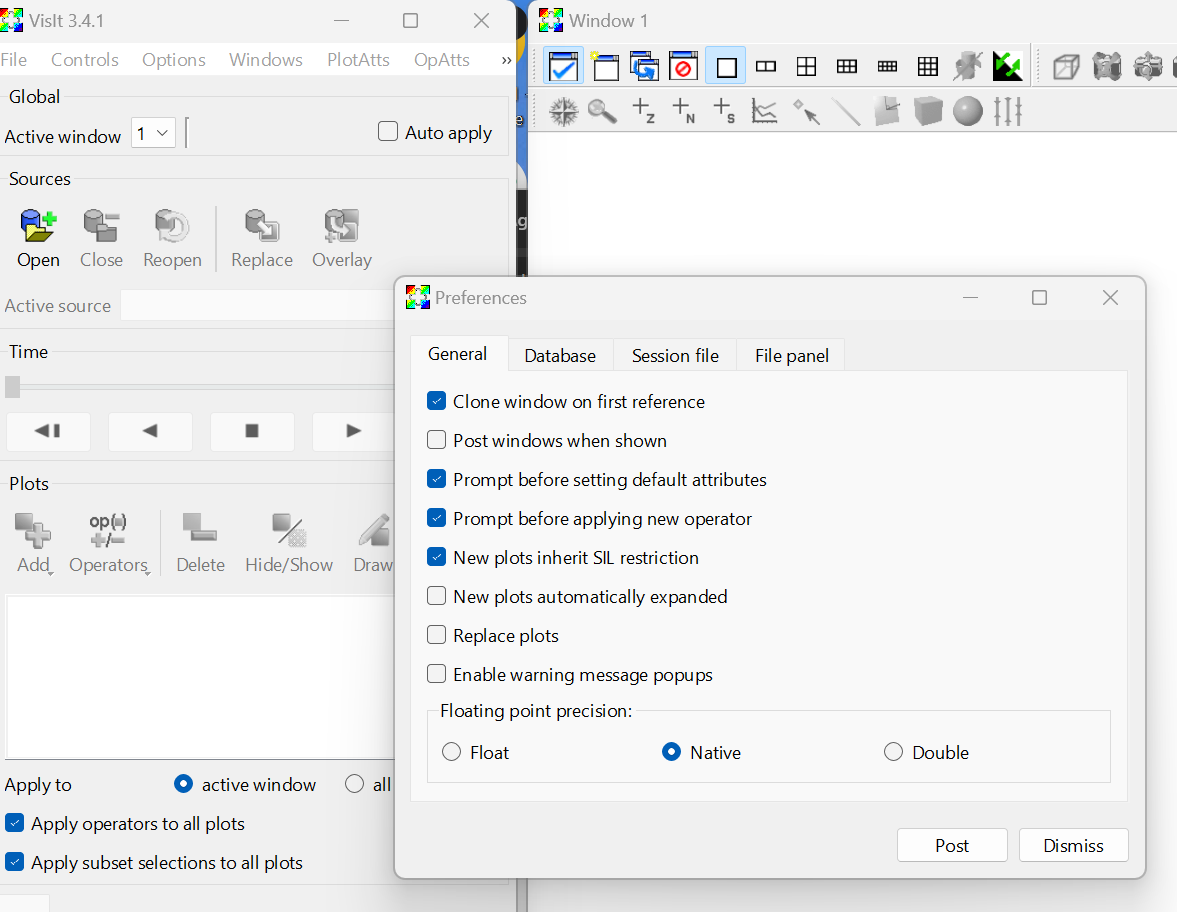
\includegraphics[width=0.88\textwidth]{ch4b-ibp-s12-preferences.png}
\scriptsize The Preferences window (3.4.1); the box to untick is the last one of the General tab.
\end{columns}
\end{frame}

\begin{frame}{Step 1: open the points}
\label{fr:open}
\begin{columns}[T]
\column{0.44\textwidth}
\footnotesize
\begin{itemize}
  \item \gui{File $\to$ Open file} (or the folder icon), go to the run's \code{viz\_IB2d} folder.
  \item With \gui{File grouping} at \gui{Smart}, the panel shows \code{lagsPts.*.vtk database (76 total files)} above the single files. Select the database line and \gui{OK}.
  \item Nothing is drawn yet: the file is open, no plot exists. The \gui{Active source} box in the main window now reads \code{lagsPts.*.vtk database}.
  \item The same works for \code{lagPtsConnect.*.vtk} (the points joined by the springs: slide \ref{fr:connect}) and for the force files in \code{hier\_IB2d\_data}.
\end{itemize}
\column{0.54\textwidth}
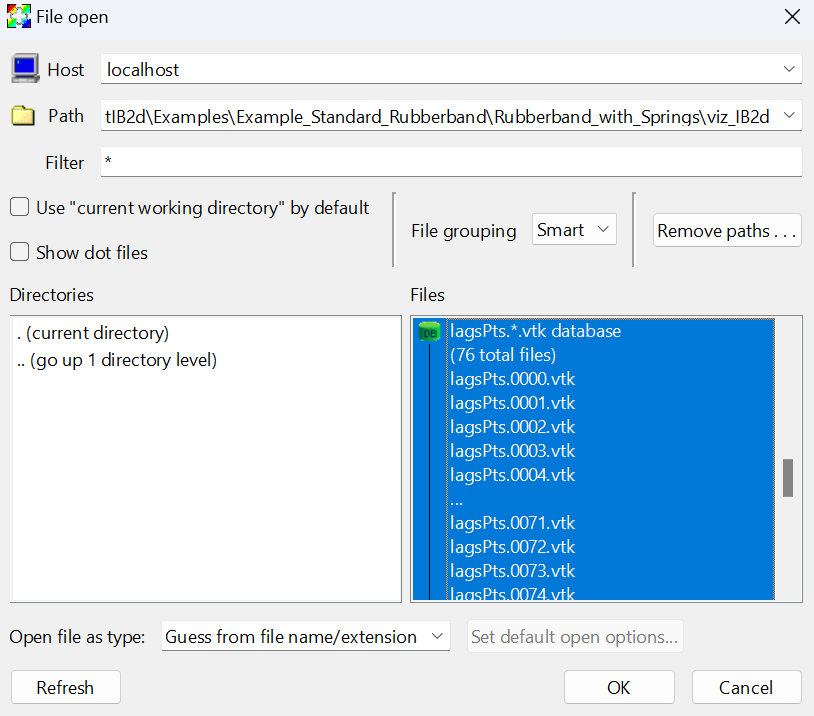
\includegraphics[width=0.9\textwidth]{ch4b-ibp-s13-open-b.png}
\scriptsize The File open window with the grouped database selected (3.4.1, Windows).
\end{columns}
\end{frame}

\begin{frame}{Step 2: add the Mesh plot, draw it, make the points visible}
\label{fr:mesh}
\begin{columns}[T]
\column{0.5\textwidth}
\small
\begin{itemize}
  \item \gui{Add $\to$ Mesh $\to$ mesh}, then \gui{Draw}. The points appear, tiny.
  \item Double-click the \gui{Mesh} entry in the plot list (or \gui{PlotAtts $\to$ Mesh}): set \gui{Point size (pixels)} to 8 and \gui{Apply} (the practical's value; chapter 26 uses 4--8 for a figure). \gui{Point type} \gui{Point} draws squares, \gui{Sphere} discs.
  \item The mesh colour can be set under \gui{Mesh color $\to$ Custom}; black prints best.
  \item Headless, the same is \code{AddPlot("Mesh", "mesh")} with \code{MeshAttributes().pointSizePixels = 8} (\code{visit\_ch4b.sh}).
\end{itemize}
\column{0.48\textwidth}
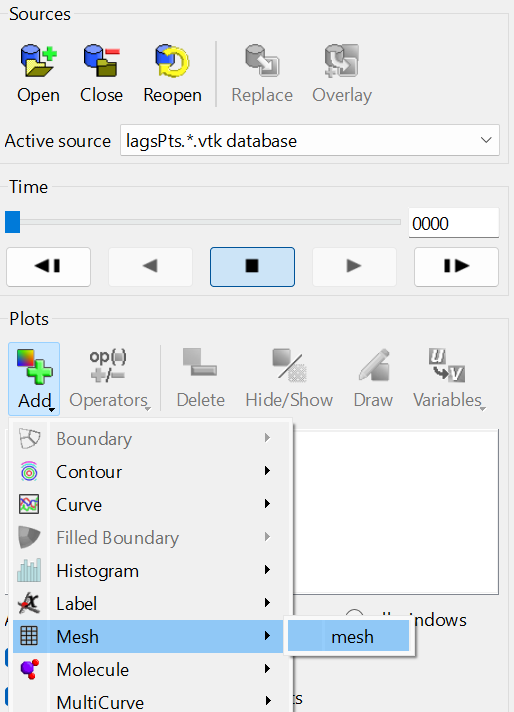
\includegraphics[width=0.48\textwidth]{ch4b-ibp-s14-add-mesh-a.png}\hfill
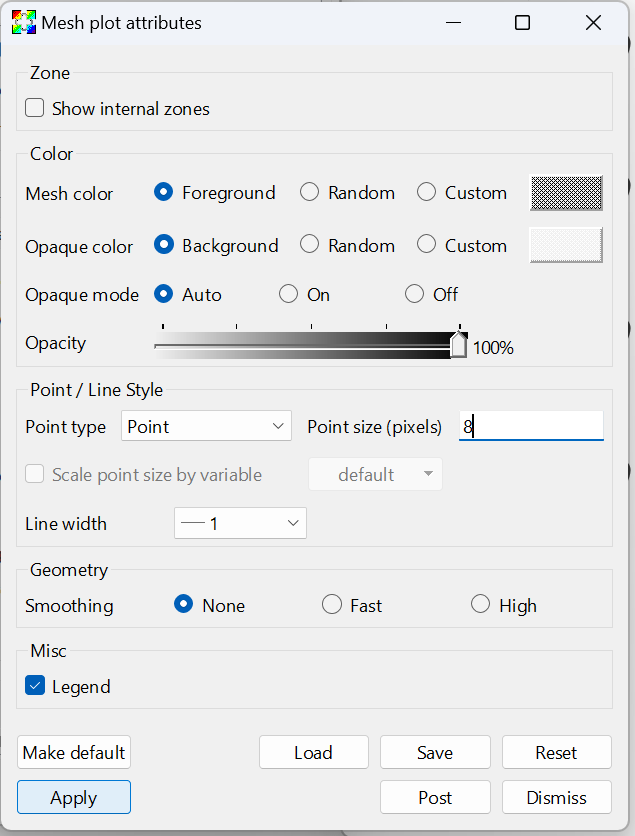
\includegraphics[width=0.48\textwidth]{ch4b-ibp-s16-mesh-attr-b.png}
\scriptsize Left: \gui{Add $\to$ Mesh}. Right: the Mesh attributes window with the point size.
\end{columns}
\end{frame}

\begin{frame}{The points, drawn}
\label{fr:pointspic}
\begin{columns}[T]
\column{0.5\textwidth}
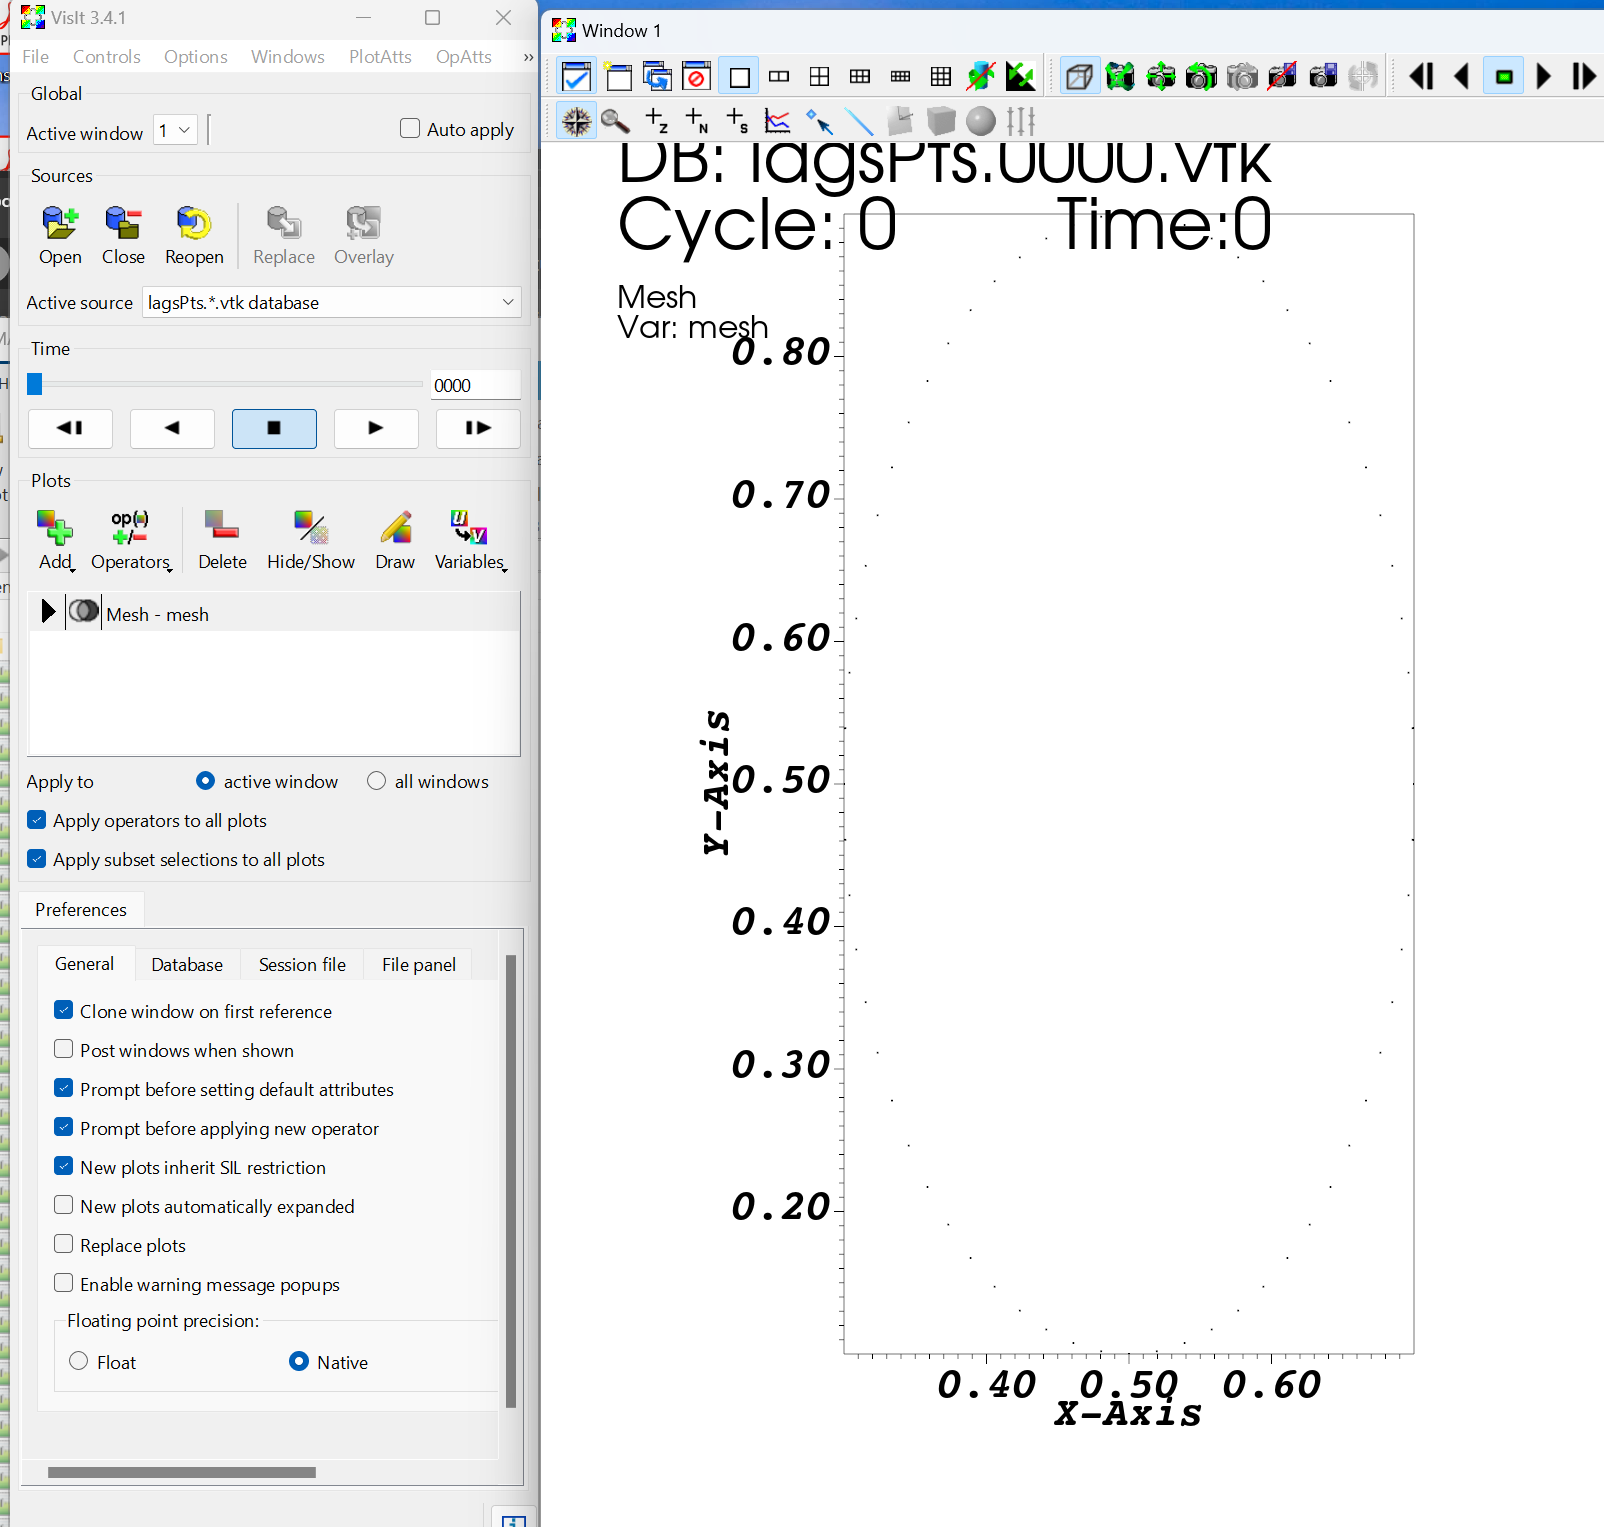
\includegraphics[width=0.78\textwidth]{ch4b-ibp-s16-mesh-attr-a.png}
\scriptsize The 2024 window: the band's 64 points at $t = 0$ as first drawn, before the point size is set (``the vertices are small, so \ldots''), with the default annotations (database name, cycle and time top left, user and date bottom right).
\column{0.48\textwidth}
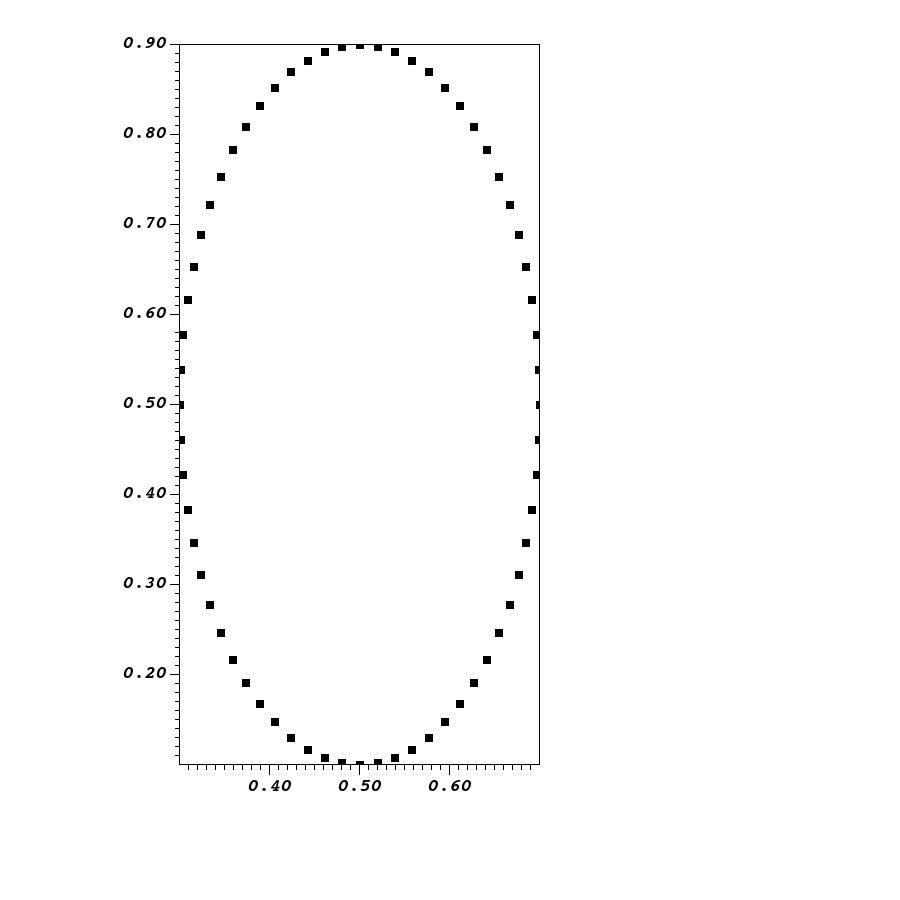
\includegraphics[width=0.78\textwidth]{ch4b-visit-points-t0.png}
\scriptsize The same state from the Python run in VisIt 3.5.0 headless, annotations off except the axes. The time of a Python-written file is its index; the MATLAB window above says \code{Time: 0}.
\end{columns}
\end{frame}

\begin{frame}{Step 3: the velocity vectors, and the correlation question}
\label{fr:correlate}
\begin{columns}[T]
\column{0.5\textwidth}
\footnotesize
\begin{itemize}
  \item \gui{Open} again and select \code{u.*.vtk database}. \gui{Add $\to$ Vector $\to$ u}.
  \item VisIt asks whether to create an \al{``Index'' database correlation} between \code{u.*.vtk database} and \code{lagsPts.*.vtk database}. \gui{Yes}: from now on one time slider moves both, state $k$ with state $k$. (\gui{No} leaves two sliders, and the points would stay at $t = 0$ while the vectors advance.)
  \item \gui{Draw}. At state 0 the velocity is zero, so nothing shows: advance with the \gui{$\triangleright$} button next to the time slider, or type a state number into it.
  \item The reset-view button (the camera with the green cross in the toolbar) shows the whole box again after a zoom or after the view has followed a plot.
\end{itemize}
\column{0.48\textwidth}
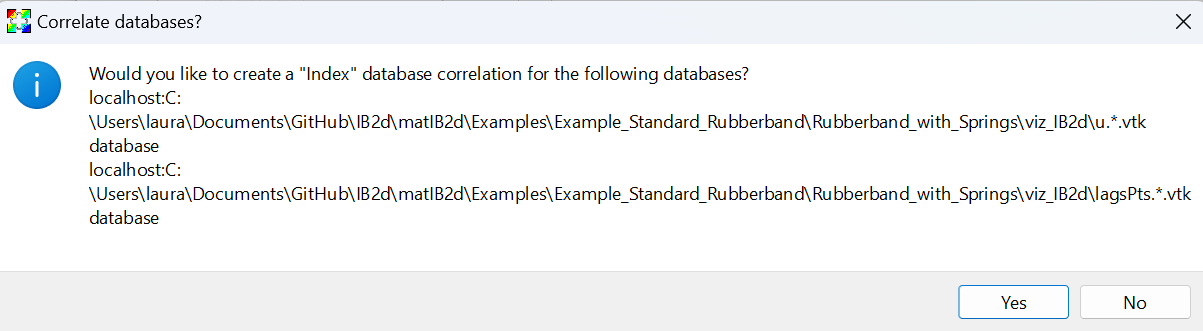
\includegraphics[width=\textwidth]{ch4b-ibp-s18-correlation.png}
\scriptsize The prompt (3.4.1). Headless: \code{CreateDatabaseCorrelation("rb", (LAG, OM), 0)} and \code{SetActiveTimeSlider("rb")}; 0 is the index method.
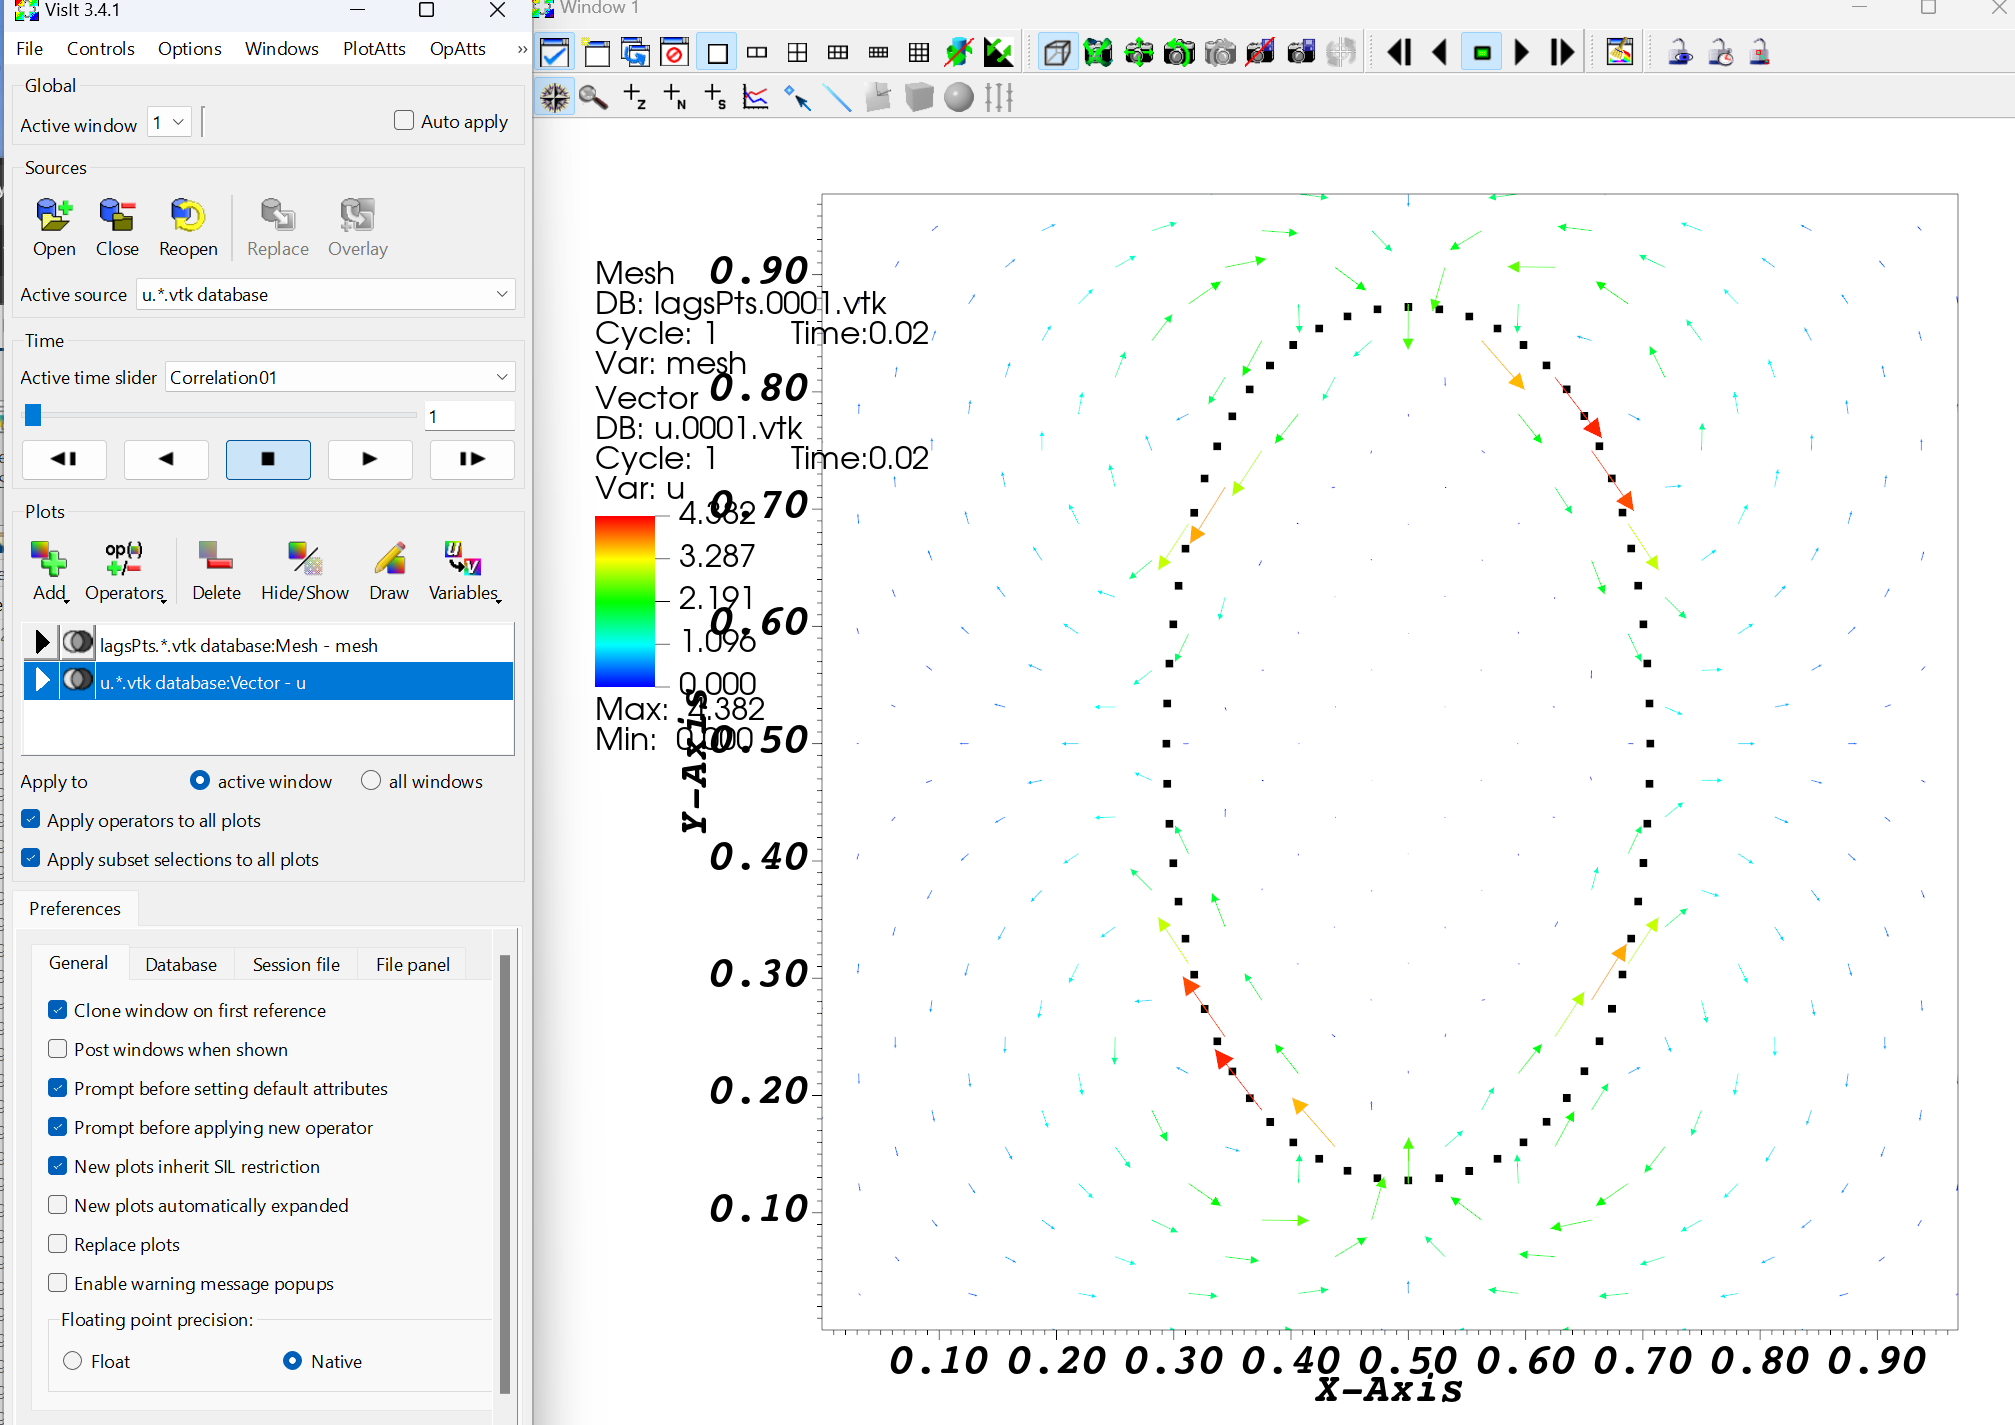
\includegraphics[width=0.6\textwidth]{ch4b-ibp-s19-advance.png}
\scriptsize The time controls and the reset-view button.
\end{columns}
\end{frame}

\begin{frame}{Step 4: the vorticity, and plots on top of plots}
\label{fr:omega}
\begin{columns}[T]
\column{0.5\textwidth}
\small
\begin{itemize}
  \item Select the \code{u} plot and \gui{Hide/Show} it (the vectors are hard to read under a colour map at first). \gui{Open} \code{Omega.*.vtk database}; \gui{Add $\to$ Pseudocolor $\to$ Omega}; \gui{Draw}; say \gui{Yes} to the correlation again.
  \item The points have disappeared: \al{VisIt draws plots in the order they were added}, and the opaque colour map covers the earlier Mesh plot. Set the \gui{Active source} back to \code{lagsPts.*.vtk database}, \gui{Add $\to$ Mesh $\to$ mesh}, \gui{Draw}: the points come back on top. (Or give the Pseudocolor an opacity below 1: next slide.)
  \item The default colour table (\code{hot}) and automatic limits change from state to state; the 2024 window at dump 1 reads $\pm 129$.
\end{itemize}
\column{0.48\textwidth}
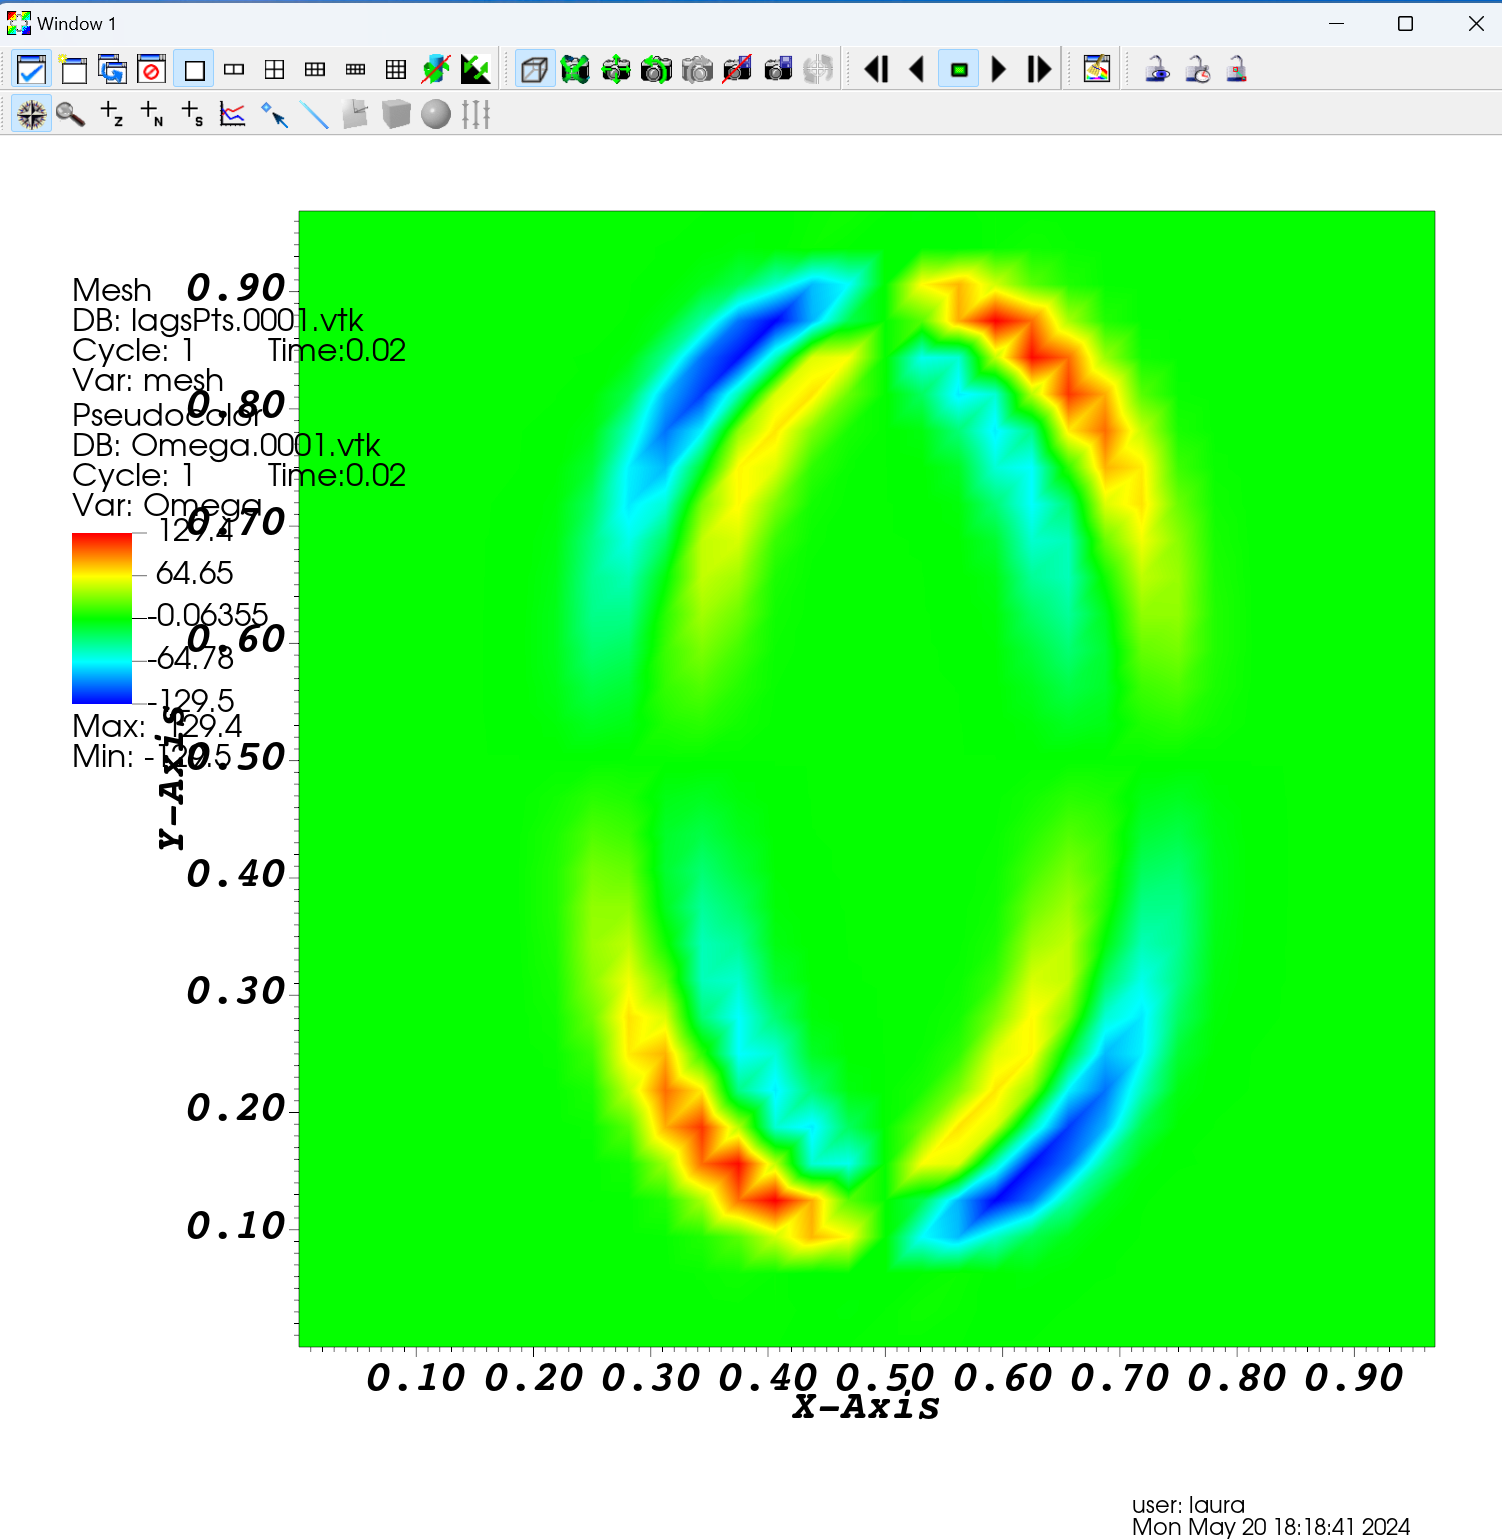
\includegraphics[width=0.78\textwidth]{ch4b-ibp-s21-vorticity-plot.png}
\scriptsize The 2024 window after \gui{Draw}: the Pseudocolor of \code{Omega} at dump 1 (\code{Time: 0.02}, the MATLAB stamp), legend with automatic limits, the points hidden underneath.
\end{columns}
\end{frame}

\begin{frame}{Step 5: make the vorticity readable (1/2)}
\label{fr:custom}
\begin{columns}[T]
\column{0.5\textwidth}
\footnotesize
Double-click the Pseudocolor entry (or \gui{PlotAtts $\to$ Pseudocolor}):
\begin{itemize}
  \item \gui{Limits}: \gui{Minimum} $-50$, \gui{Maximum} $50$. The practical: ``these are just approximate values''. They clip the peaks (129 at dump 1; above 50 in 57 of the 76 dumps) and show the shear layers at one scale, which is what makes frames comparable (chapter 26); the extremes at states 15 and 75 are $\pm 52$ and $\pm 58$ (the \gui{MinMax} query, slide \ref{fr:query}).
  \item \gui{Centering}: \gui{Nodal}. Harmless here: IB2d writes its fields as point data, which VisIt already treats as nodal (a headless render with and without the setting is pixel-identical); the step matters for IBAMR's zone-centred vorticity, where it came from (chapter 26).
\end{itemize}
\column{0.48\textwidth}
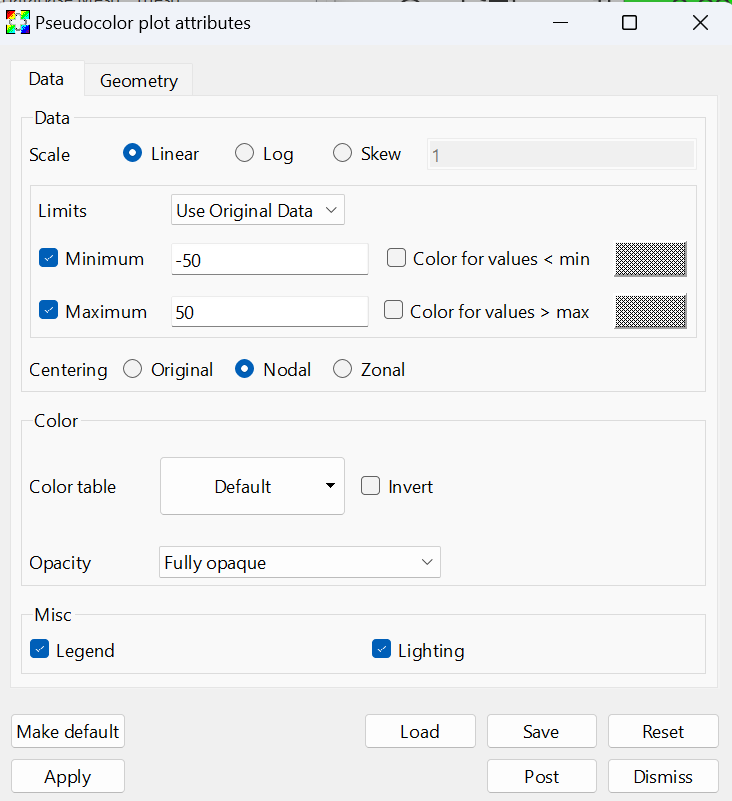
\includegraphics[width=0.52\textwidth]{ch4b-ibp-s22-pseudocolor-attr.png}
\scriptsize The Pseudocolor attributes window (3.4.1): limits, centering, opacity.
\end{columns}
\end{frame}

\begin{frame}{Step 5: make the vorticity readable (2/2)}
\label{fr:custom2}
\begin{columns}[T]
\column{0.5\textwidth}
\footnotesize
\begin{itemize}
  \item \gui{Opacity}: \gui{Constant}, then 70\,\% on the slider (the 3.4.1 window shows the drop-down at \gui{Fully opaque}), so that the vectors and points show through.
  \item A diverging colour table (\code{difference}, blue--white--red) reads better than \code{hot} for a signed field; chapter 26's advice.
  \item \gui{Apply}; then \gui{Hide/Show} the vectors again, and press \gui{Play}: ``the rubberband bounding [sic] with the formation of new vortices during each bounce''.
\end{itemize}
\column{0.48\textwidth}
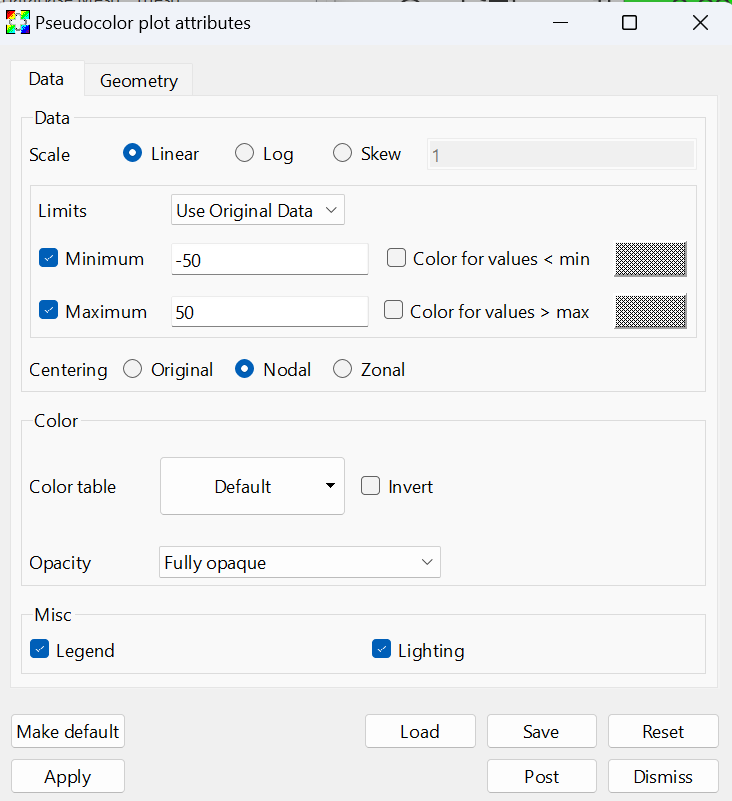
\includegraphics[width=0.52\textwidth]{ch4b-ibp-s22-pseudocolor-attr.png}
\scriptsize The Pseudocolor attributes window (3.4.1): limits, centering, opacity.
\end{columns}
\end{frame}

\begin{frame}{The result: four states of the Python run in VisIt 3.5}
\label{fr:result}
\begin{columns}[T]
\column{0.24\textwidth}
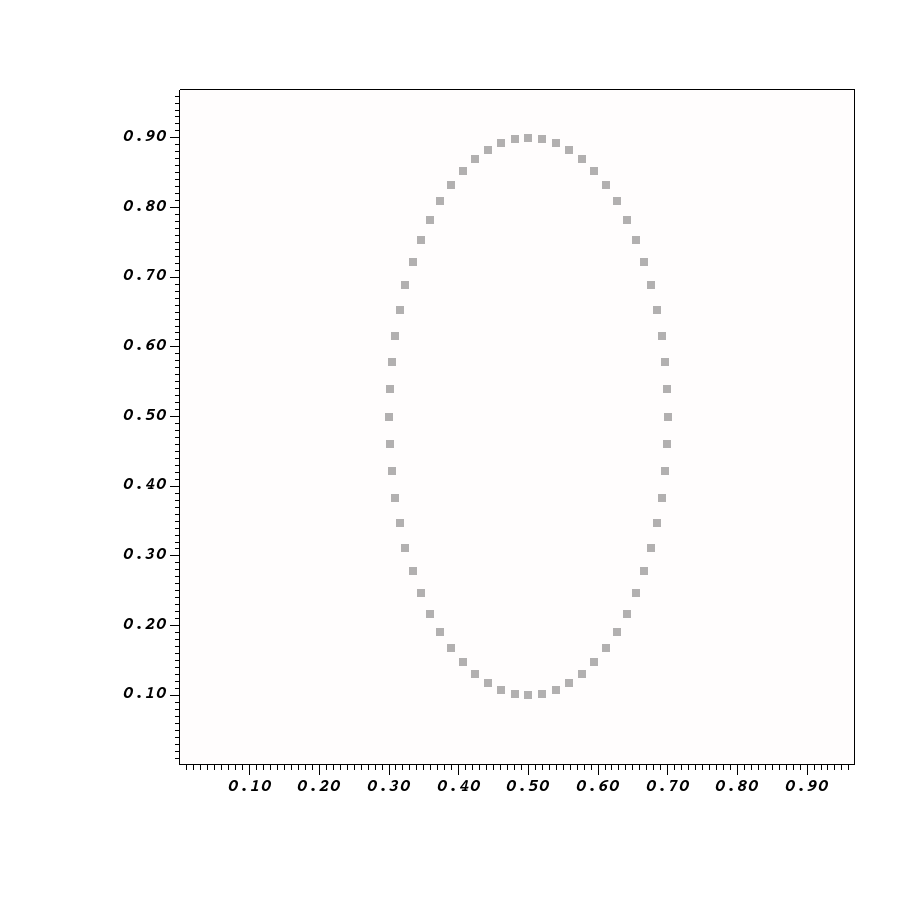
\includegraphics[width=\textwidth]{ch4b-visit-omega-0000.png}
\column{0.24\textwidth}
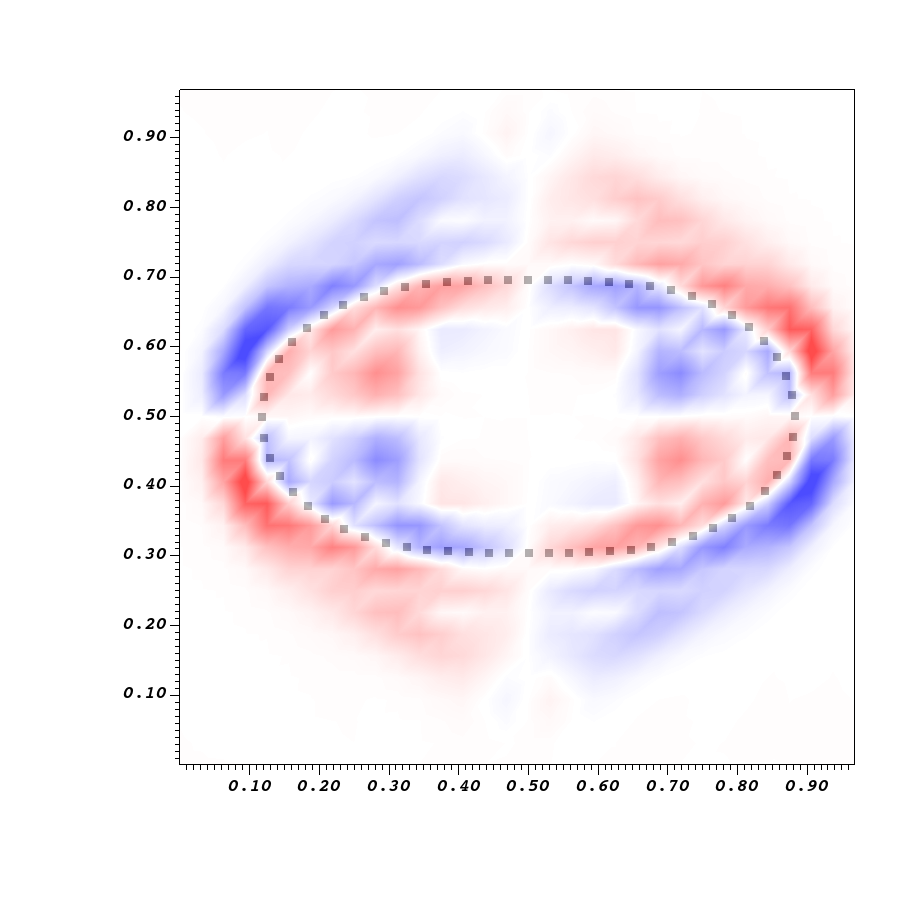
\includegraphics[width=\textwidth]{ch4b-visit-omega-0005.png}
\column{0.24\textwidth}
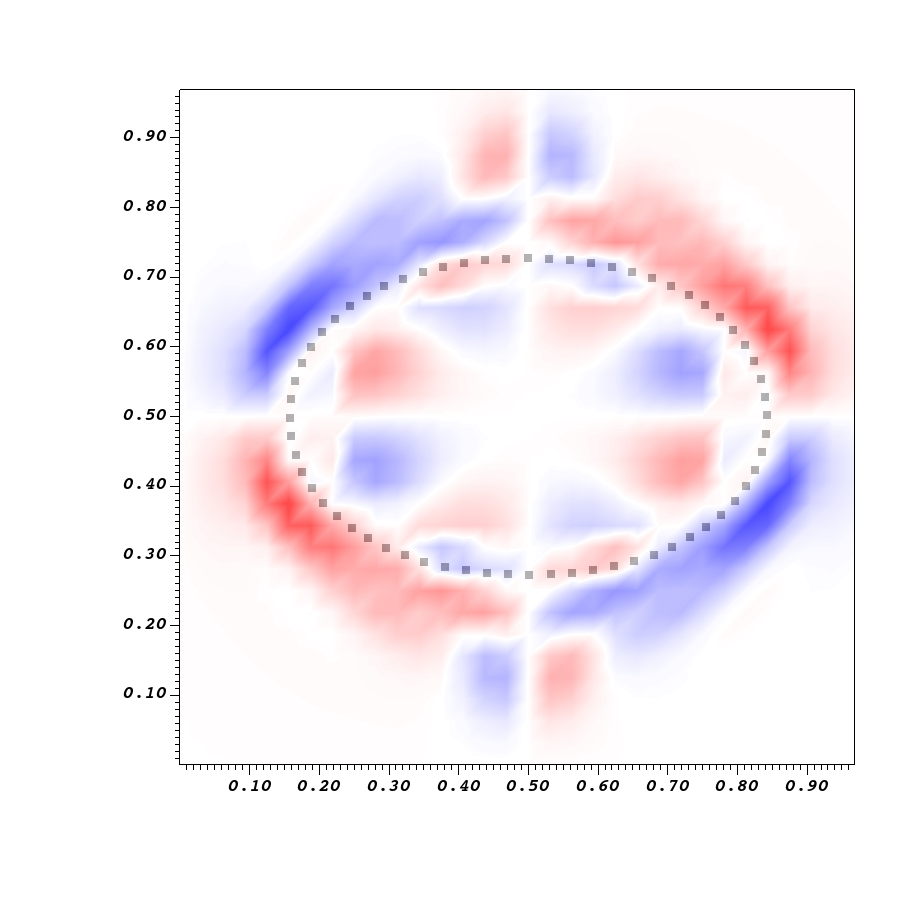
\includegraphics[width=\textwidth]{ch4b-visit-omega-0015.png}
\column{0.24\textwidth}
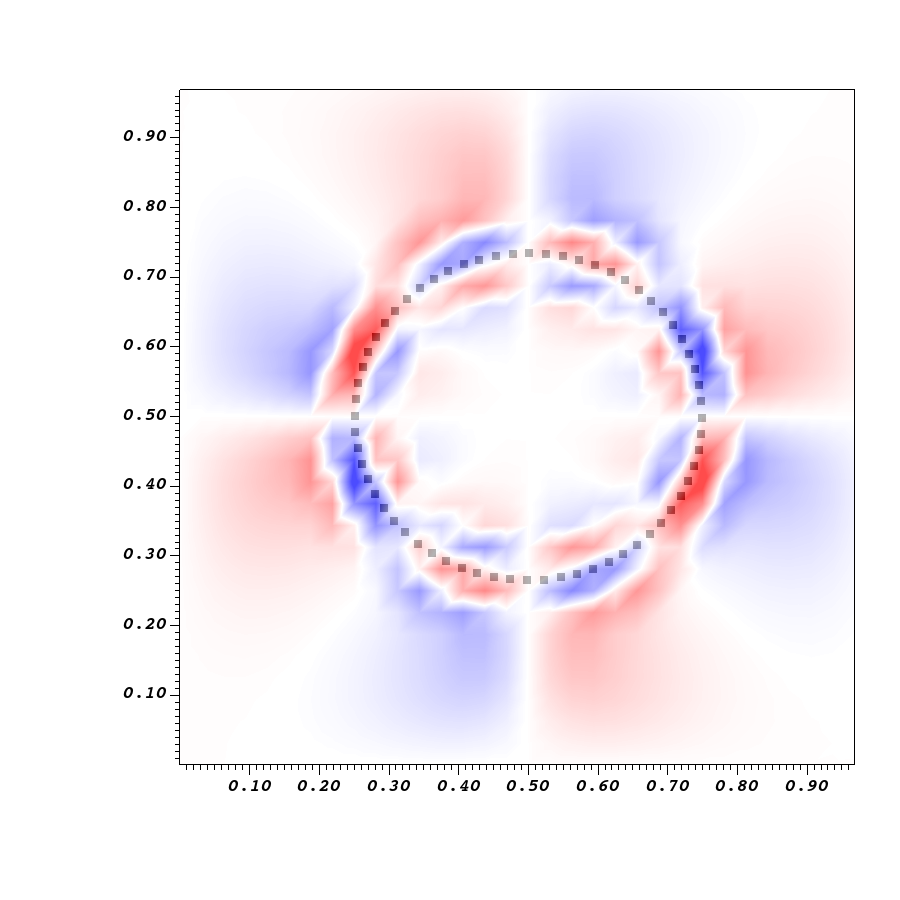
\includegraphics[width=\textwidth]{ch4b-visit-omega-0075.png}
\end{columns}
\small States 0, 5, 15 and 75 ($t = 0$, 0.1, 0.3, 1.5 s): Pseudocolor of \code{Omega}, limits $\pm 50$, nodal, 70\,\% opacity, \code{difference} colour table; the Mesh plot of the points added before it, which is why the points look grey through the colour map. Compare chapter 4a's matplotlib frames of the same files.
\begin{itemize}
  \item At state 0 the field is zero everywhere (a uniform white): the fluid starts at rest and the band has not yet pulled.
  \item The four corner vortices and the thin shear layers along the band are the same at every resolution; their strength is not (chapter 4d).
\end{itemize}
\end{frame}

\begin{frame}{Vectors and colour together}
\label{fr:vectors}
\begin{columns}[T]
\column{0.4\textwidth}
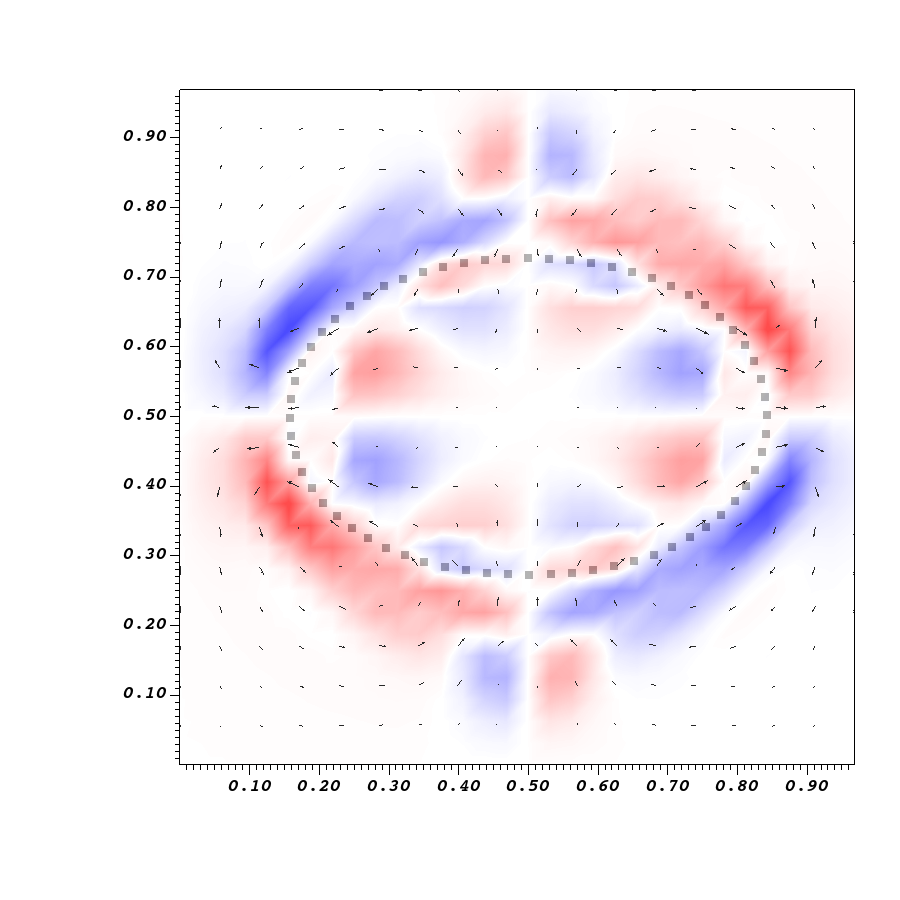
\includegraphics[width=\textwidth]{ch4b-visit-omega-u-0015.png}
\scriptsize State 15 with the Vector plot of \code{u} (600 vectors, uniform in space, scaled by magnitude) on top of the vorticity.
\column{0.58\textwidth}
\footnotesize
\begin{itemize}
  \item The Vector plot's attributes (\gui{Vectors}: uniformly located, a number such as 600 at $32^2$ and 8000 at $512^2$; \gui{Scale} and \gui{Scale by magnitude}; \gui{Color}: constant) are chapter 26's; the practical leaves the defaults.
  \item VisIt 3.5 prints \gui{The Vector plot of variable ``u'' yielded no data} when the plot is drawn at state 0 (the field is zero) and draws it anyway at the other states; chapter 26 notes the same warning. Not an error.
  \item The peak speed at state 15 is 1.59 (the \gui{MinMax} query on the Vector plot); 4.5 over the whole run (chapter 4a).
\end{itemize}
\end{columns}
\end{frame}

\begin{frame}{The connected points}
\label{fr:connect}
\begin{columns}[T]
\column{0.4\textwidth}
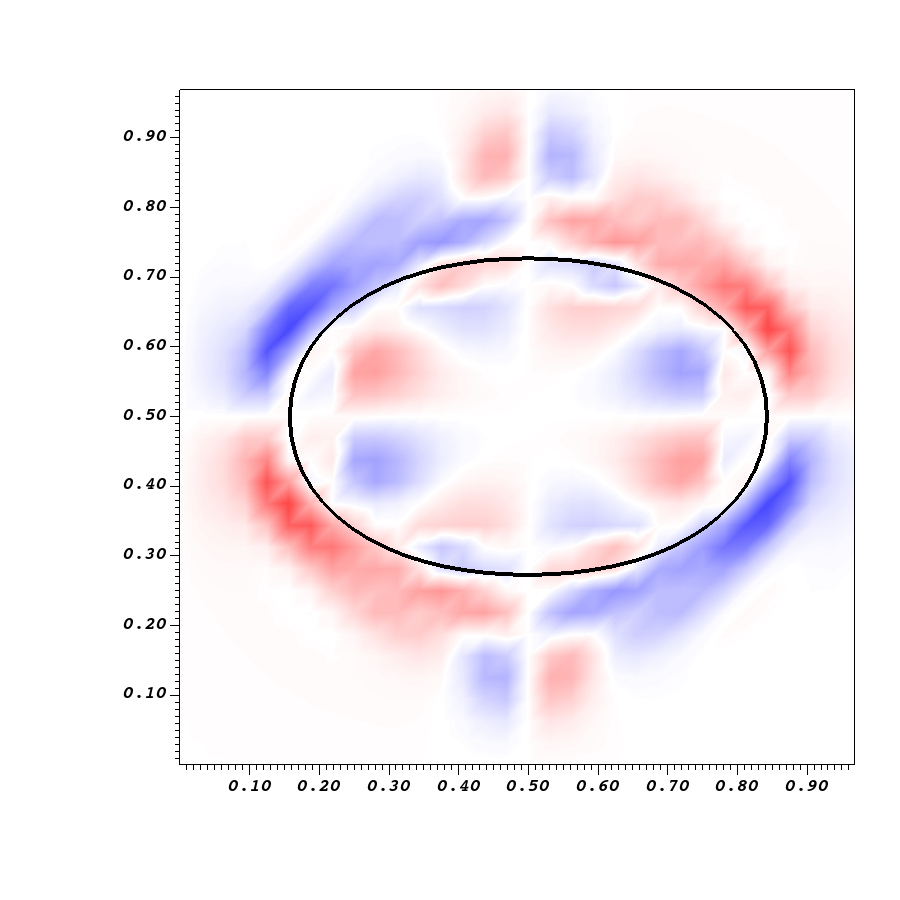
\includegraphics[width=\textwidth]{ch4b-visit-connect-0015.png}
\column{0.58\textwidth}
\small
\begin{itemize}
  \item \code{lagPtsConnect.*.vtk} holds the same points joined into line segments along the springs (and only the springs: without \code{springs = 1} no connection file is written, as \code{Wobbly\_Beam}'s output shows): a Mesh plot of it with \gui{Line width} 3 draws the band as a curve (left, state 15 over the vorticity), the choice for figures.
  \item Open it like \code{lagsPts}: \code{lagPtsConnect.*.vtk database}, \gui{Add $\to$ Mesh $\to$ mesh}, line width in the Mesh attributes, and the same ``Index'' correlation.
  \item For an open structure (a beam, the heart tube's two walls) the segments follow the spring list, so a wall drawn this way shows gaps exactly where springs are missing: a second geometry check.
\end{itemize}
\end{columns}
\end{frame}

\begin{frame}{Queries: a number from the window}
\label{fr:query}
\small
\begin{itemize}
  \item \gui{Controls $\to$ Query} (chapter 26): \gui{MinMax} on the active Pseudocolor gives the extremes with their node and position; on the Vector plot it gives the speed. At state 15: \code{Omega -- Min = -51.49 (node 411 at <0.84375, 0.375>)}, \code{Max = 52.21}; \code{u -- Max = 1.59 (node 516 at <0.125, 0.5>)}.
  \item \gui{Pick} on a point (chapter 28) prints its coordinates and, for the force databases, the force; the points have no variables of their own in \code{lagsPts}.
  \item \gui{Lineout} across the band gives a profile of \code{Omega} or \code{uMag} as a curve, with the time slider still working (chapter 26's Lineout; chapter 29 for the analysis).
  \item For a number against time (a tip's position, the peak force, a flow rate), chapter 33's readers do it in a few lines from the files; chapter 4a's half-width plot and the forces plot of slide \ref{fr:forces} are that.
\end{itemize}
\begin{punchbox}
\small The query must be made on the plot that holds the variable (select it in the plot list first); on the Mesh plot VisIt answers ``Cannot perform a MinMax query on variable mesh.''
\end{punchbox}
\end{frame}

\begin{frame}{Zoom, annotations, sessions}
\label{fr:zoom}
\begin{columns}[T]
\column{0.5\textwidth}
\footnotesize
\begin{itemize}
  \item \al{Zoom}: the magnifying glass in the toolbar, then drag a box in the window; the reset-view button restores the whole box. (The practical's sentence ``the region of interest, namely that around the channel and cavities'' is left over from the IBAMR deck it was adapted from.)
  \item \al{Annotations} (chapter 26, slide on annotations): \gui{Controls $\to$ Annotation}: untick \gui{Database} and \gui{User information} for a clean figure; the \gui{2D} tab for axis titles and fonts; the \gui{Objects} tab to drop the legend's title and min/max and to move it.
\end{itemize}
\column{0.48\textwidth}
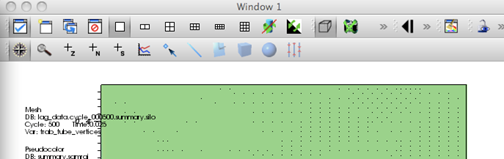
\includegraphics[width=\textwidth]{ch4b-ibp-s24-zoom.png}
\scriptsize The zoom and reset-view buttons (a VisIt 2.5.2 window reused by the 2024 practical).
\end{columns}
\end{frame}

\begin{frame}{Sessions and saving a window}
\label{fr:sessions}
\small
\begin{itemize}
  \item \al{Sessions}: \gui{File $\to$ Save session} keeps every plot and setting; \gui{Restore session} reopens them; \gui{Restore session with sources} points the same session at another run's files (Lecture 10). Save one once the window looks right.
  \item \al{Save window}: \gui{File $\to$ Save window} writes a PNG of the current state at the size set under \gui{File $\to$ Set save options}.
  \item A session file is text (XML) and travels with the run: keep it next to \code{viz\_IB2d} so that the figure can be remade after the next run.
\end{itemize}
\end{frame}

\begin{frame}[fragile]{A movie}
\label{fr:movie}
\begin{columns}[T]
\column{0.5\textwidth}
\small
\begin{itemize}
  \item The practical's route: \gui{File $\to$ Save movie}, \gui{New simple movie}, format \gui{MPEG movie}, the \gui{$\to$} button, then the frame range, frame rate, stride, folder and name. It works; Lecture 10 calls it ``not the best option''.
  \item The better route (chapter 30): the same wizard with format \gui{PNG} writes one frame per state; join them with ffmpeg (next slide).
\end{itemize}
\column{0.48\textwidth}
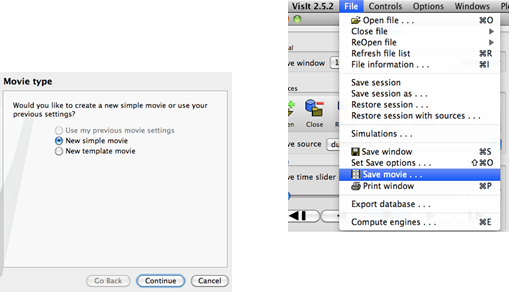
\includegraphics[width=0.75\textwidth]{ch4b-ibp-s25-save-movie.png}

\vspace{1mm}
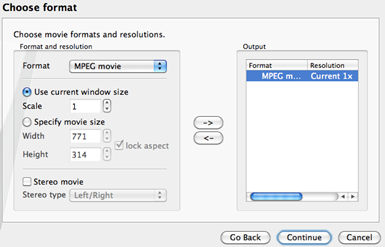
\includegraphics[width=0.6\textwidth]{ch4b-ibp-s26-movie-format.png}
\scriptsize The Save movie wizard's first two screens (2024 practical).
\end{columns}
\end{frame}

\begin{frame}[fragile]{Frames and ffmpeg}
\label{fr:ffmpeg}
\begin{lstlisting}[style=shell]
ffmpeg -framerate 10 -i rubberband%04d.png -pix_fmt yuv420p -vf "scale=trunc(iw/2)*2:trunc(ih/2)*2" rubberband.mp4
\end{lstlisting}
\small
\begin{itemize}
  \item Lecture 10 named ``VirtualDub (free for PC) or Quicktime Pro'' for the joining; ffmpeg is free on all three systems (\code{apt install ffmpeg}, Homebrew, or the Windows build) and scriptable.
  \item Headless, \code{SaveWindow()} in a loop over \code{SetTimeSliderState(k)} writes the frames without the GUI (chapter 32; \code{visit\_ch4b.sh} saves four of them that way).
  \item The \code{-vf scale} part keeps both dimensions even, which the H.264 encoder requires; \code{-framerate 10} shows 76 frames in 7.6 s. Chapter 30 has the options (frame rate, size, a title frame, GIF).
\end{itemize}
\end{frame}

\begin{frame}[fragile]{The same steps as a script (what chapter 32 teaches)}
\label{fr:script}
\begin{columns}[T]
\column{0.56\textwidth}
\begin{lstlisting}[style=py,basicstyle=\ttfamily\tiny\color{BlackGray}]
LAG = RUN + "/viz_IB2d/lagsPts.*.vtk database"
OM  = RUN + "/viz_IB2d/Omega.*.vtk database"
OpenDatabase(LAG)
AddPlot("Mesh", "mesh")
m = MeshAttributes(); m.pointSizePixels = 8; m.legendFlag = 0
m.meshColor = (0, 0, 0, 255); m.meshColorSource = m.MeshCustom; SetPlotOptions(m)
OpenDatabase(OM); ActivateDatabase(OM)
AddPlot("Pseudocolor", "Omega")
pc = PseudocolorAttributes(); pc.minFlag = pc.maxFlag = 1; pc.min, pc.max = -50, 50
pc.centering = pc.Nodal; pc.opacityType = pc.Constant; pc.opacity = 0.7
pc.colorTableName = "difference"; SetPlotOptions(pc)
CreateDatabaseCorrelation("rb", (LAG, OM), 0)   # the "Index" correlation
SetActiveTimeSlider("rb"); DrawPlots()
for k in (0, 5, 15, 75):
    SetTimeSliderState(k); DrawPlots()
    SetActivePlots(1); print(k, Query("MinMax"))
    s = SaveWindowAttributes(); s.fileName = "ch4b-visit-omega-%04d" % k
    s.family = 0; s.format = s.PNG; SetSaveWindowAttributes(s); SaveWindow()
\end{lstlisting}
\column{0.42\textwidth}
\small
\begin{itemize}
  \item Run with \code{visit -nowin -cli -s script.py} (no window) or \code{visit -cli -s script.py} (with one). This is how the pictures of slides \ref{fr:pointspic}--\ref{fr:connect} were made.
  \item Every button of the walk-through has a line here; \gui{Controls $\to$ Command} records the lines as you click (chapter 32).
  \item The Mesh plot is added first and is plot 0; the Pseudocolor is plot 1, the one the query needs (\code{SetActivePlots(1)}).
  \item The full script, with the vectors and the connected points, is \code{wsl/final/visit\_ch4b.sh}.
\end{itemize}
\end{columns}
\end{frame}

% ---------------------------------------------------------------- forces
\begin{frame}{The forces on the structure: \code{hier\_IB2d\_data}}
\label{fr:forces}
\begin{center}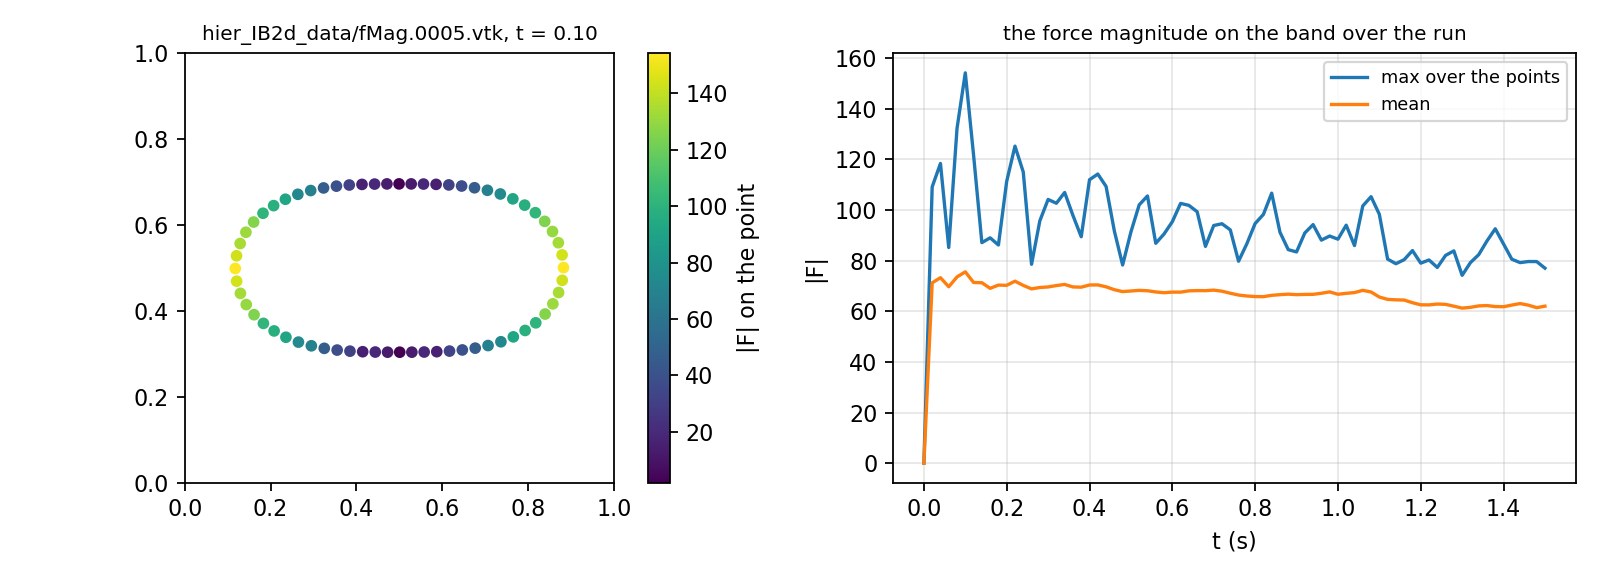
\includegraphics[width=0.62\textwidth]{ch4b-forces.png}\end{center}
\footnotesize
\begin{itemize}
  \item \code{fMag.NNNN.vtk} in \code{hier\_IB2d\_data} is the magnitude of the force each point exerts on the fluid, as a scalar on the points; \code{fX\_Lag}, \code{fY\_Lag} are its components. Left: dump 5 ($t = 0.1$), when the force peaks (154 at the sides of the band, where the springs are most stretched); right: its maximum and mean over the points against time (the mean is 71 at the first dump, 76 at its peak and 62 at the end, as the band relaxes).
  \item In VisIt: open \code{fMag.*.vtk database}, \gui{Add $\to$ Pseudocolor $\to$ fMag}, and the points colour by force (set the point size as before). From the files: chapter 33's \code{read\_vtk\_legacy} gives the points and the \code{fMag} array; the plot above is that, in Python.
  \item The sum of \code{fX\_Lag} over the points is the net force on the fluid, the quantity chapter 11 computes for drag and lift in IBAMR; the same bookkeeping applies here.
\end{itemize}
\end{frame}

% ---------------------------------------------------------------- part C: more examples
\begin{frame}{Four more Python examples, run as shipped (October 2026)}
\label{fr:more}
\scriptsize
\begin{tabular}{@{}L{0.21\textwidth}L{0.29\textwidth}L{0.12\textwidth}L{0.08\textwidth}L{0.13\textwidth}@{}}
\toprule
example (\code{pyIB2d/Examples}) & models (\code{input2d}) & grid, $\Delta t$, $T$ & wall & output \\
\midrule
\code{Wobbly\_Beam} & beams + 2 target points (a curved beam held at both ends, straightening) & $32^2$, $5 \cdot 10^{-5}$, 0.05 & 2.7 s & 100 dumps \\
\code{Single\_Porous\_}\allowbreak\code{Rubberband} & springs + porous points (\code{.porous}) & $32^2$, $10^{-4}$, 0.1 & 3.2 s & 100 dumps, 11 files each \\
\code{HeartTube\_}\allowbreak\code{Muscle} & springs + beams + target points + muscles (\code{.muscle}, activation in \code{give\_Muscle\_Activation.py}) & $128^2$, $5 \cdot 10^{-4}$, 0.25 & 14 s & 50 dumps \\
\code{Tracers\_In\_}\allowbreak\code{Impedance\_Pump} & springs updated in time (\code{update\_Springs.py}) + beams + target points + 110 tracers & $64^2$, $10^{-3}$, 2 & 53 s (after a fix) & 401 dumps, with \code{tracer} files \\
\bottomrule
\end{tabular}

\vspace{1mm}
\footnotesize
\begin{itemize}
  \item All four print their models under ``FIBER MODEL INCLUDES'' (the heart tube: Springs, Beams, Target Pts, ``MUSCLE MODEL (Force-Velocity / Length-Tension Model)''); none needs anything beyond chapter 4a's set-up.
  \item \code{Rubberband\_with\_Beams} needs the \code{input2d} fix of chapter 4a before it does anything; the pump needs a one-line fix in the driver (slide \ref{fr:pumpfix}).
  \item The VisIt steps are the same for every one of them; the pictures that follow are matplotlib on the files, as in chapter 4a.
\end{itemize}
\end{frame}

\begin{frame}{The porous band}
\label{fr:porous}
\begin{center}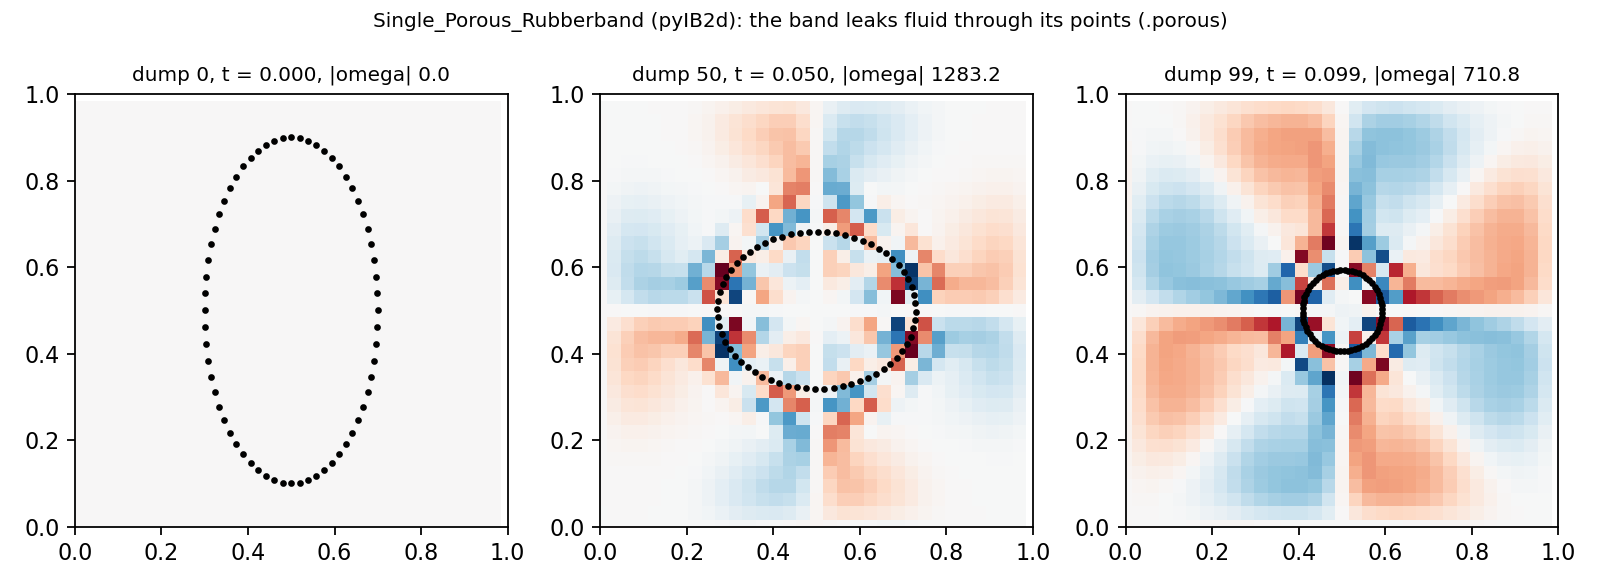
\includegraphics[width=0.78\textwidth]{ch4b-porous-frames.png}\end{center}
\footnotesize
\begin{itemize}
  \item \code{Single\_Porous\_Rubberband}: a 64-point band with a \code{.porous} file (a porosity coefficient per point) and springs 400 times stiffer than the springs example's ($k = 10^7$). Each point slips through the fluid in proportion to the force on it (\code{please\_Compute\_Porous\_Slip\_Velocity}), so the band leaks and shrinks fast ($x$ half-width 0.09 by $t = 0.1$). Do not compare it with the springs run of chapter 4a (different stiffness); the MATLAB folder \code{Example\_Porous\_Rubberbands} has the side-by-side comparison with a sealed band at the same $k$.
  \item 1000 steps of $10^{-4}$ (the stiff springs set the time step; chapter 4d): 3.2 s, 100 dumps every 10 steps, 11 files per dump (\code{uX}, \code{uY}, \code{fX}, \code{fY}, \code{fMag} switched on in this \code{input2d}).
\end{itemize}
\end{frame}

\begin{frame}{The heart tube with muscles}
\label{fr:hearttube}
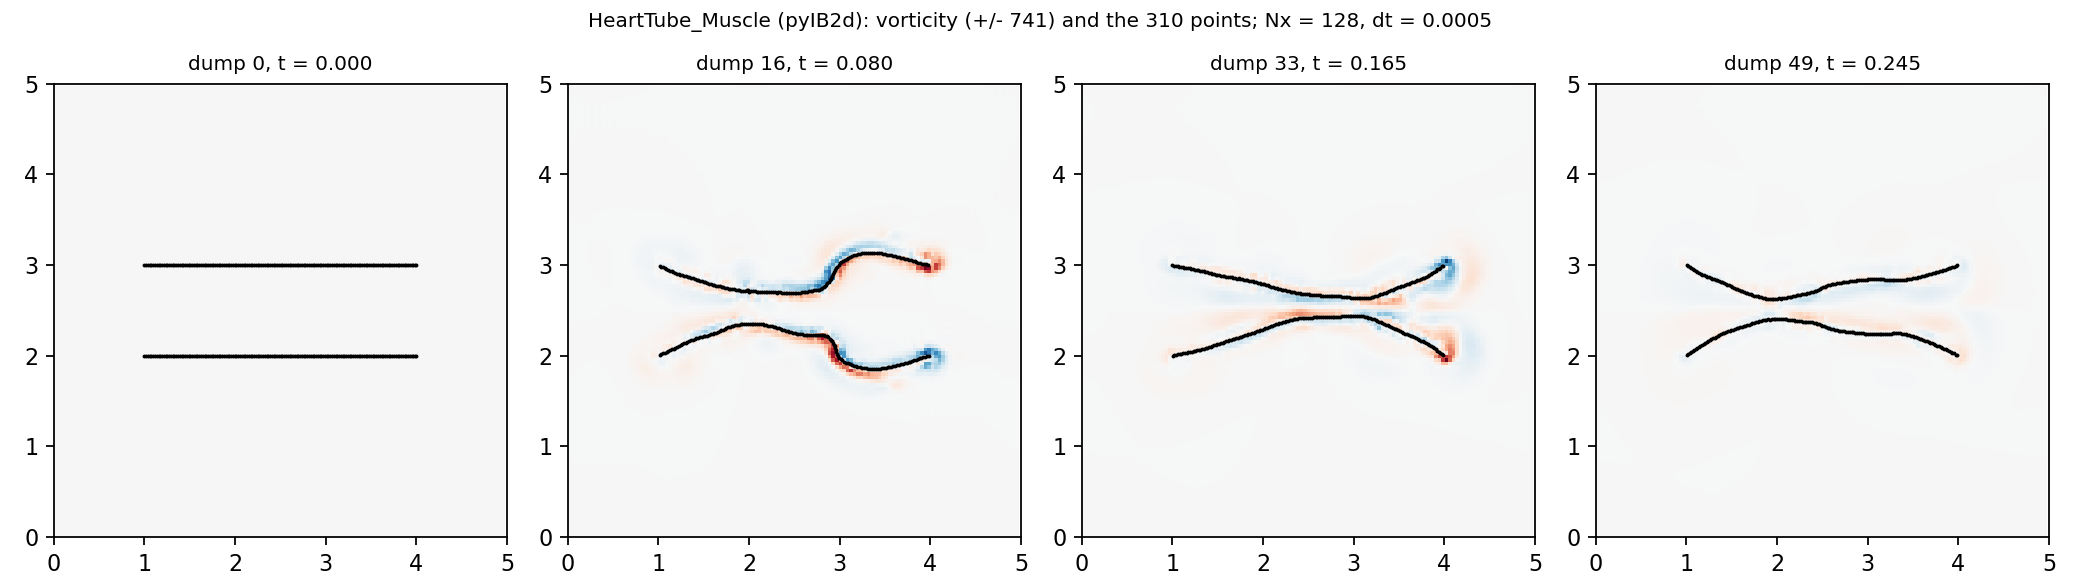
\includegraphics[width=\textwidth]{ch4b-hearttube-frames.png}
\footnotesize
\begin{itemize}
  \item \code{HeartTube\_Muscle}: two walls of a tube (310 points) held by target points at the ends, with springs and beams along them and muscle fibres across (\code{HeartTube.muscle}, the force-velocity/length-tension model of the 2015 paper); \code{give\_Muscle\_Activation.py} sends a wave of activation along the tube and the walls pinch in turn. \code{test\_Activation\_Wave.py} plots that wave without running anything.
  \item $128^2$, 500 steps: 14 s, 50 dumps. The frames are scaled to $\pm 741$, the largest value among the four shown; the run's peak is $3.5 \cdot 10^3$ in the first dump, a start-up transient on the walls. The muscle model, its parameters and what the tube pumps are chapter 4e's.
\end{itemize}
\end{frame}

\begin{frame}{The impedance pump with tracers}
\label{fr:pump}
{\centering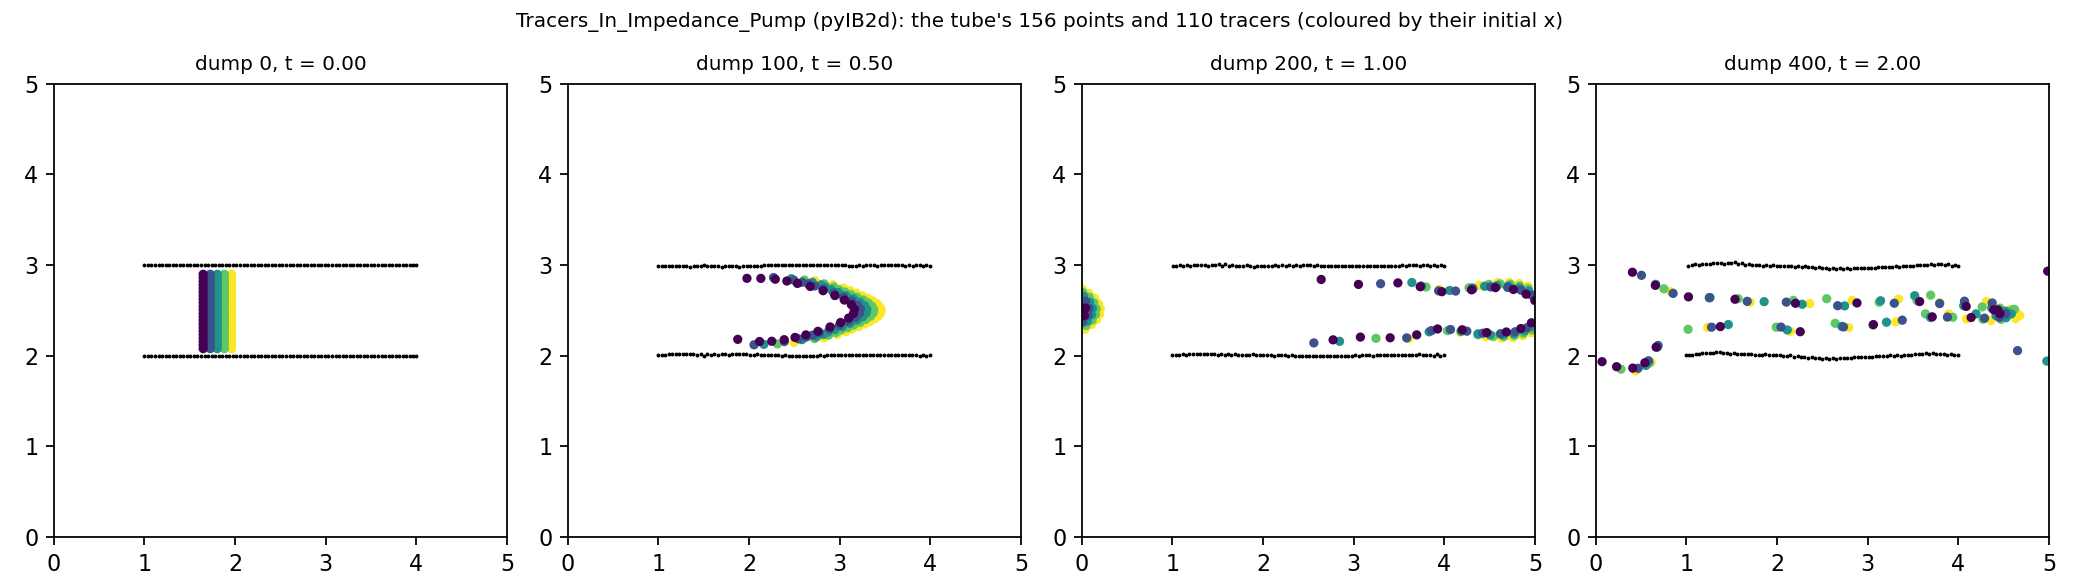
\includegraphics[width=0.88\textwidth]{ch4b-pump-tracers.png}\par}
\footnotesize
\begin{itemize}
  \item \code{Tracers\_In\_Impedance\_Pump}: a tube of 156 points whose springs change their resting lengths in time (\code{update\_Springs.py}, chapter 4c) to pinch one section periodically; 110 passive tracers (\code{HeartTube.tracer}) ride the flow and show the net transport: their mean $x$ moves from 1.80 to 2.81 in 2 s, and that understates the transport, because tracers that reach the right edge re-enter at the left (the periodic box; visible in the last frame). The tube is 3 long in a box of 5. An impedance pump moves fluid without valves by pinching off-centre (chapter 4e; the IBAMR heart-tube pump is IB/11, chapter 9b; the two-point valveless pump is chapter 36).
  \item $64^2$, 2000 steps: 53 s, 401 dumps every 5 steps, 12 files each (the \code{tracer.NNNN.vtk} files are the tracers' positions; VisIt opens them like the points).
\end{itemize}
\end{frame}

\begin{frame}[fragile]{The pump example as shipped stops at the first step}
\label{fr:pumpfix}
\begin{columns}[T]
\column{0.5\textwidth}
\small
In the 2024 clone, \code{python3 main2d.py} in \code{Tracers\_In\_Impedance\_Pump} writes dump 0000 and dies:
\begin{lstlisting}[style=tiny]
  File ".../IBM_Blackbox/IBM_Driver.py", line 821, in main
    xT, yT = please_Move_Lagrangian_Point_Positions(Uh, Vh, xT, yT, xT, yT,
TypeError: please_Move_Lagrangian_Point_Positions() missing 4 required positional arguments: 'porous_Yes', 'poroelastic_Yes', 'poroelastic_info', and 'F_Poro'
\end{lstlisting}
The tracer branch of the driver calls the point mover with the signature it had before the porous and poroelastic arguments were added (and without \code{mu}); the two calls for the structure itself were updated, this one was not. Any Python example with \code{tracers = 1} fails the same way.
\column{0.48\textwidth}
\small
The fix, in \code{pyIB2d/IBM\_Blackbox/IBM\_Driver.py} at that line (the tracers are never porous):
\begin{lstlisting}[style=tiny]
xT, yT = please_Move_Lagrangian_Point_Positions(mu, Uh, Vh, xT, yT, xT, yT,
    x, y, dt, grid_Info, 0, 0, 0, 0)
\end{lstlisting}
\begin{itemize}\setlength{\itemsep}{0pt}
  \item With it the example runs to the end (53 s) and the tracers move as on the previous slide.
  \item Like the \code{nonInv\_beams} key of chapter 4a and the \code{fNorm}/\code{fTan} test, this is worth a note to the IB2d repository; the MATLAB version has no such problem (its driver passes the full argument list).
  \item The lesson is chapter 4a's: a run that starts is not a run that finished. Count the dumps.
\end{itemize}
\end{columns}
\end{frame}

\begin{frame}{The swimmer (MATLAB): a beam that changes its curvature}
\label{fr:swimmer}
\begin{columns}[T]
\column{0.46\textwidth}
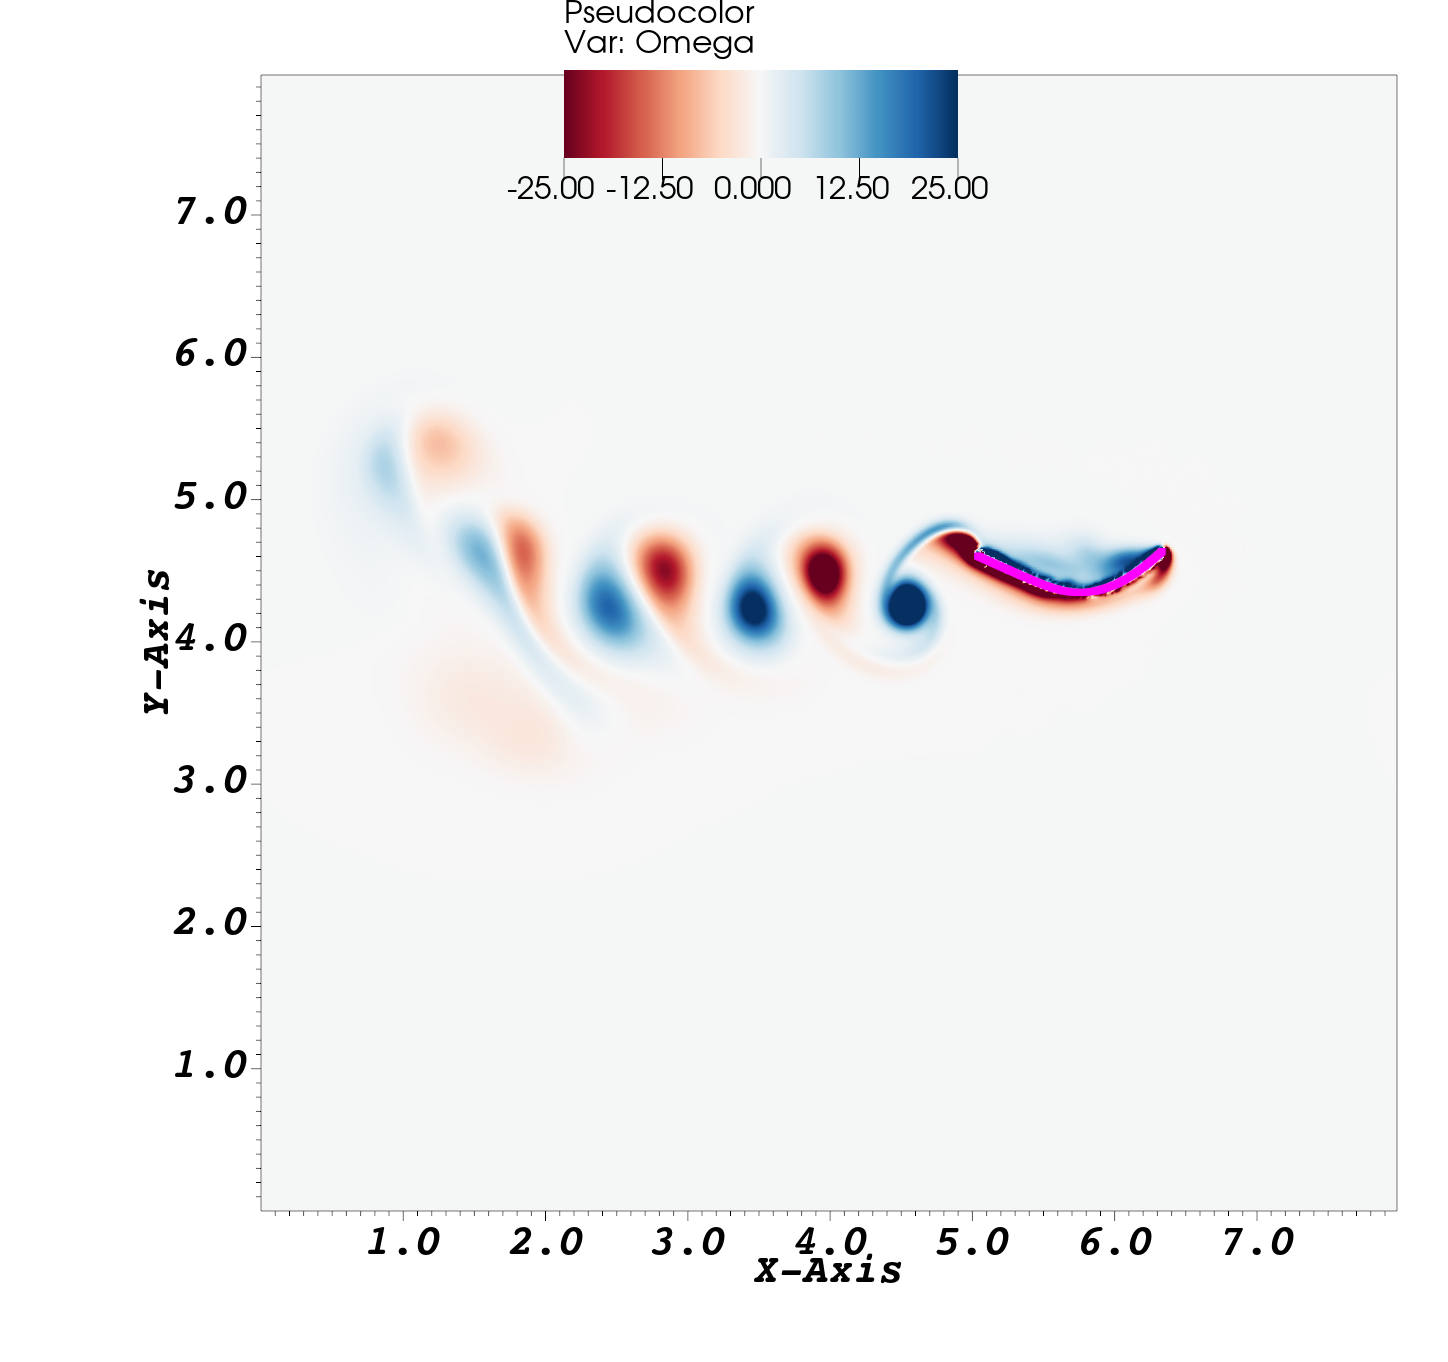
\includegraphics[width=0.47\textwidth]{ch4b-ibp-s34-swimmer-start.png}\hfill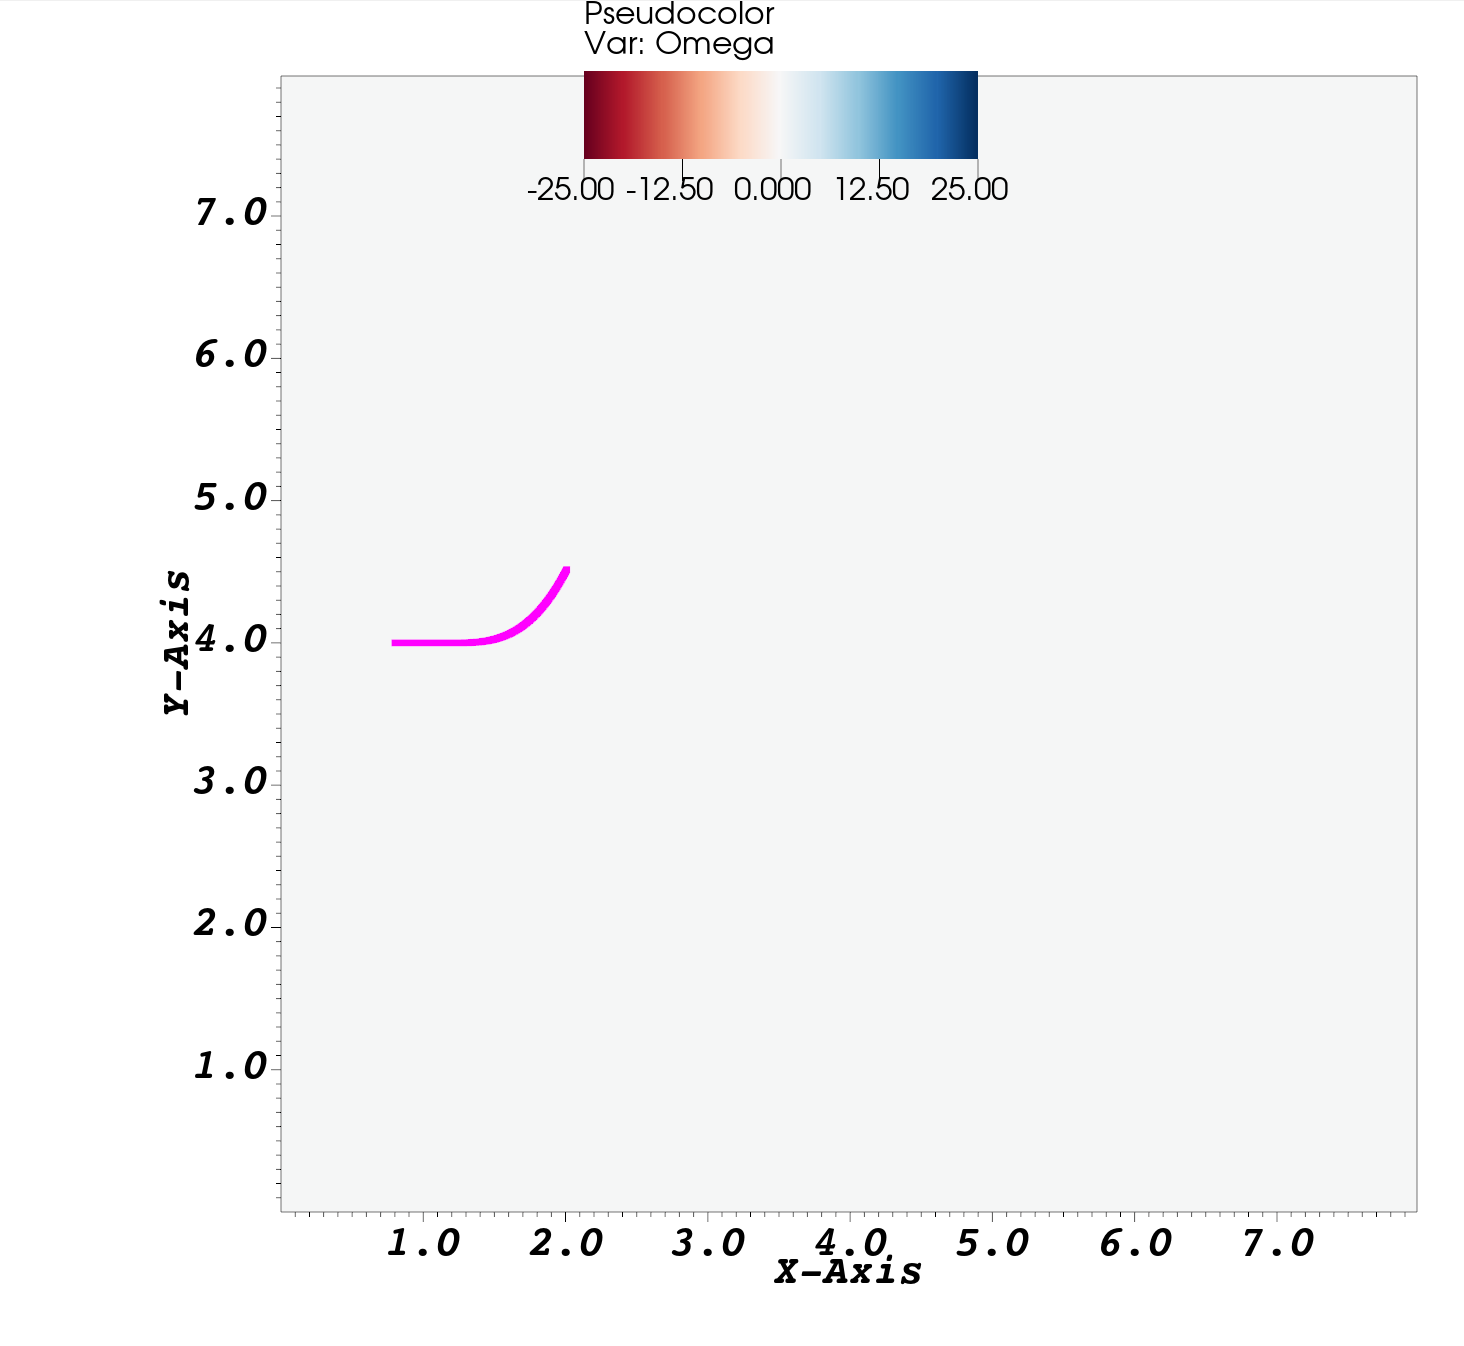
\includegraphics[width=0.47\textwidth]{ch4b-ibp-s34-swimmer-end.png}

\scriptsize Start and end of the run (2024 practical).
\column{0.52\textwidth}
\small
\begin{itemize}
  \item \code{matIB2d/Examples/}\allowbreak\code{Examples\_First\_Year\_Seminar/}\allowbreak\code{Swimmer}: $512^2$ on an $8 \times 8$ box, $\Delta t = 2.5 \cdot 10^{-5}$, $T = 3$. ``about 15-20 mins to get to time 1'' (the practical); run it, watch, and stop it with Ctrl-C when you have seen enough.
  \item A line of points with springs and non-invariant beams whose preferred curvature changes in time: the swimming comes from the fluid. Chapter 4c builds a smaller version of exactly this mechanism.
\end{itemize}
\end{columns}
\end{frame}

\begin{frame}{The swimmer's files}
\label{fr:swimmer2}
\small
The files, and what each does (the practical's slides 31--33):
\begin{itemize}
  \item \code{Swimmer\_Geometry.m} writes \code{swimmer.vertex}, \code{.spring}, \code{.nonInv\_beam}: a line of points with springs and non-invariant beams (chapter 4a).
  \item \code{swimmer.phases} stores the $x$ and the two $y$ profiles of the swimmer's two phases; \code{test\_Script.m} reads it and displays the motion without running the fluid.
  \item \code{update\_nonInv\_Beams.m} is called every step (\code{update\_nonInv\_beams = 1}): it takes the time within the period ($t = $ \code{rem(current\_time, period)}, period 0.5 s as a 0.25 s down-stroke and a 0.25 s up-stroke), interpolates between the two phases with a piecewise quadratic--cubic--quadratic blend (coefficients \code{a}, \code{b}, \code{c}, \code{d}, \code{g}, \code{h} in the file), computes the curvatures as second differences, and writes the new $C_x$, $C_y$ into columns 5 and 6 of the beam table.
  \item The curvature is prescribed, the position is not: the beam's forces and the fluid decide where the swimmer goes.
\end{itemize}
\end{frame}

\begin{frame}{The leaf (MATLAB): a structure that releases a scalar into a flow}
\label{fr:leaf}
\begin{columns}[T]
\column{0.4\textwidth}
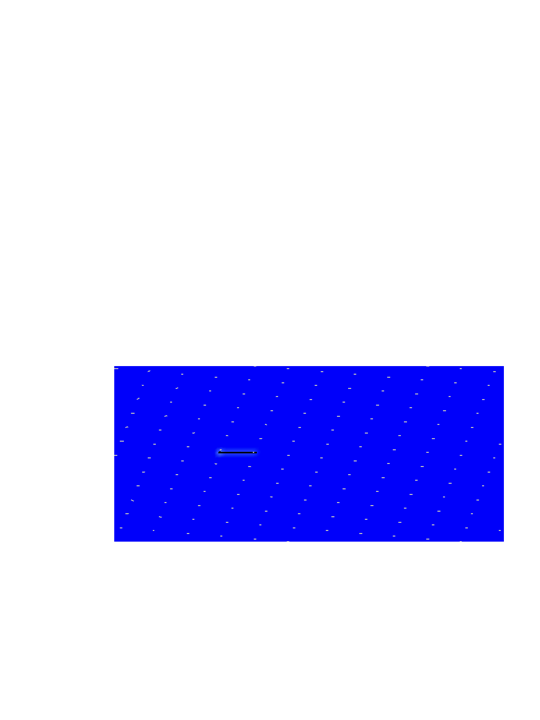
\includegraphics[width=0.47\textwidth]{ch4b-ibp-s38-leaf-start.png}\hfill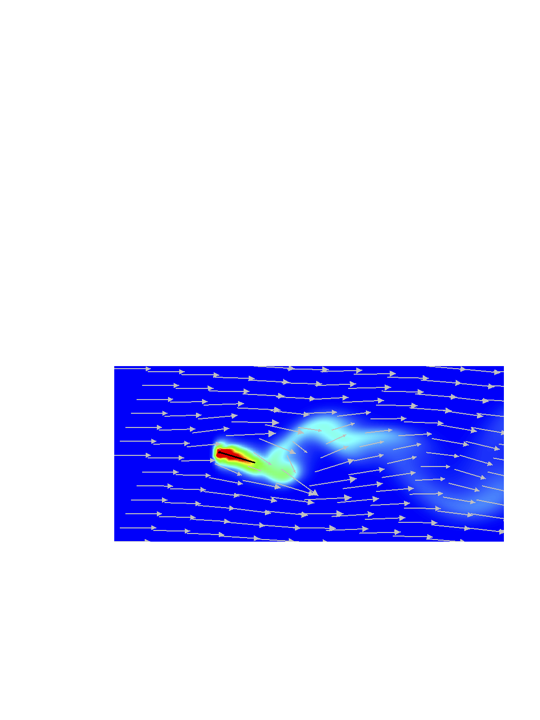
\includegraphics[width=0.47\textwidth]{ch4b-ibp-s38-leaf-end.png}

\scriptsize Start and end (2024 practical): the leaf on its stem in the channel, the concentration it sheds.
\column{0.58\textwidth}
\small
\begin{itemize}
  \item \code{matIB2d/Examples/}\allowbreak\code{Example\_Concentration\_Dynamics/}\allowbreak\code{Leaf\_64}: a $384 \times 64$ grid on a $30 \times 5$ box, $\Delta t = 5 \cdot 10^{-5}$, $T = 3.25$; a cylinder (the stem) held by target points with a flexible line (the leaf) attached, built from \code{leaf.vertex}, \code{.spring}, \code{.beam}, \code{.mass}, \code{.target}, plus \code{leaf.concentration}, the initial scalar field.
\end{itemize}
\end{columns}
\end{frame}

\begin{frame}{The leaf's files}
\label{fr:leaf2}
\small
\begin{itemize}
  \item \code{Leaf\_Leaf.m} writes the files; \code{give\_me\_source\_model.m} is the source of the scalar on the leaf; \code{please\_Compute\_External\_Forcing.m} sets the background flow entering on the left (\code{arb\_ext\_force = 1}: the ``pseudo-inflow'' of chapter 4a).
  \item The practical calls the scalar heat on one slide and oxygen on the next; in the code it is a passive concentration (the 2022 paper), and either reading is fine.
  \item A $384 \times 64$ run of 65\,000 steps is hours in MATLAB; it is here to be read and to show what the concentration machinery does. The IBAMR counterpart with advection--diffusion is chapter 24.
\end{itemize}
\end{frame}

\begin{frame}{Where to go from these examples}
\label{fr:where}
\small
\begin{itemize}
  \item \al{Chapter 4c} (moving boundaries): the update functions these examples use (\code{update\_Springs}, \code{update\_Target\_Point\_Positions}, \code{update\_nonInv\_Beams}) written from scratch on the sawtooth channel, and your own geometry.
  \item \al{Chapter 4d} (stability and convergence): what happens to the rubber band when $\Delta t$ doubles or the stiffness is multiplied by ten (the ``BLOW UP'' message), and the same run at $32^2$, $64^2$ and $128^2$.
  \item \al{Chapter 4e} (the gallery, the muscle models): the heart tube's muscle law, the pumps, the mass-and-gravity races, the porous bands, the Boussinesq and concentration examples, with the pictures and movies of the 2016 talk.
  \item \al{Chapter 4f} (MeshmerizeMe): a drawing into \code{.vertex} files.
  \item \al{Part V} for VisIt beyond this walk-through: chapter 26 (making it look better), 28 (the points and their variables), 29 (data analysis), 30 (movies), 31 (VisIt on the cluster), 32 (the command line and Python), 33 (the files in Python and MATLAB).
\end{itemize}
\end{frame}

% ---------------------------------------------------------------- exercises, summary
\begin{frame}{Exercises}
\label{fr:exercises}
\small
\begin{enumerate}
  \item The practical's two: change the band so that it is stretched in $y$ instead of $x$ (``enough that you can see it''), and change the viscosity in \code{input2d} to put the band in a very viscous fluid. Plot the initial state and the first dump after it with the points, the vectors and the vorticity (homework 4 of Lecture 11), and say in two sentences how the viscous run differs.
  \item Save a VisIt session of the finished window; restore it with sources on the viscous run's folder.
  \item Make a 76-frame movie of the vorticity with fixed limits, as PNG frames joined by ffmpeg; note the file size against the wizard's MPEG.
  \item From \code{hier\_IB2d\_data}, plot the maximum of \code{fMag} against time for the springs band and for the damped-springs band of chapter 4a on the same axes.
  \item Run \code{HeartTube\_Muscle} and open it in VisIt: a Pseudocolor of \code{uMag} with the connected points; find the time of the strongest pinch from the \gui{MinMax} query over the states.
  \item Apply the one-line fix of slide \ref{fr:pumpfix} and run the pump; with chapter 33's reader, plot the mean $x$ of the tracers against time, unwrapping the jumps of tracers that cross the periodic edge, and read off the pumping speed.
\end{enumerate}
\end{frame}

\begin{frame}{Summary}
\label{fr:summary}
\small
\begin{itemize}
  \item A run is \code{main2d} in an example folder; MATLAB shows a live figure, Python can; both leave \code{viz\_IB2d} (fields, points) and \code{hier\_IB2d\_data} (forces), one file per dump and variable.
  \item In VisIt, open the grouped database (\code{lagsPts.*.vtk database}), add a Mesh plot, draw, set the point size; open \code{u.*.vtk} and \code{Omega.*.vtk} the same way, accept the ``Index'' correlation so that the sliders move together, add the Vector and Pseudocolor plots; re-add the points on top; fixed limits, nodal, 70\,\% opacity; play, zoom, save a window or frames.
  \item MATLAB's files carry a time stamp, Python's an index; everything else about the files is the same in the two versions.
  \item The forces on the points are scalars on the same point files; one number per dump, plotted against time, is the usual result.
  \item Four Python examples run in seconds to a minute (one after a one-line fix); the swimmer and the leaf are MATLAB examples to read for the update functions and the concentration machinery.
  \item Next: chapter 4c moves the boundaries.
\end{itemize}
\end{frame}

\begin{frame}{References and credits}
\label{fr:refs}
\scriptsize
\begin{itemize}
  \item The IB2d repository, \url{https://github.com/nickabattista/IB2d}: \code{pyIB2d/Examples/\{Rubberband\_with\_Springs, Wobbly\_Beam, Single\_Porous\_Rubberband, HeartTube\_Muscle, Tracers\_In\_Impedance\_Pump\}}, \code{matIB2d/Examples/Examples\_First\_Year\_Seminar/Swimmer}, \code{matIB2d/Examples/Example\_Concentration\_Dynamics/Leaf\_64}, the writers in \code{IBM\_Driver.m/.py} (\code{print\_vtk\_files}, \code{savevtk\_*}); the README's VisIt note for macOS. Code as of the 2024-03-06 clone.
  \item VisIt 3.5.0 (\url{https://visit-dav.github.io/visit-website/}): the headless script \code{wsl/final/visit\_ch4b.sh} and the metadata check \code{ch4b\_facts.sh}; the runs \code{wsl/final/ib2d\_pyrun3.sh}, \code{ib2d\_pump2.sh}; the figures \code{tools/ch4b\_figures.py}, \code{ch4b\_figures2.py}, with \code{examples/analysis/read\_vtk\_legacy.py}.
  \item Sources merged (slide \ref{fr:sources}): ``IB2d Practical'' (2024; its 25 screenshots are reused here as \code{ch4b-ibp-*.png}: VisIt 3.4.1 on Windows, with a few older VisIt 2.x windows among them); ``ib2d part 2'' (Lecture 10, 2021, edited 2023); ``A quick intro to ib2d'' (Lecture 9); N. Battista's video tutorial 4. The 2015, 2017, 2018 and 2022 IB2d papers (chapter 4a's list) for the muscle, porous, tracer and concentration machinery.
  \item FFmpeg (\url{https://ffmpeg.org}), version 6.1 in the WSL used here.
\end{itemize}
\end{frame}

\end{document}
